% Template for PLoS
% Version 3.5 March 2018
%
% % % % % % % % % % % % % % % % % % % % % %
%
% -- IMPORTANT NOTE
%
% This template contains comments intended
% to minimize problems and delays during our production
% process. Please follow the template instructions
% whenever possible.
%
% % % % % % % % % % % % % % % % % % % % % % %
%
% Once your paper is accepted for publication,
% PLEASE REMOVE ALL TRACKED CHANGES in this file
% and leave only the final text of your manuscript.
% PLOS recommends the use of latexdiff to track changes during review, as this will help to maintain a clean tex file.
% Visit https://www.ctan.org/pkg/latexdiff?lang=en for info or contact us at latex@plos.org.
%
%
% There are no restrictions on package use within the LaTeX files except that
% no packages listed in the template may be deleted.
%
% Please do not include colors or graphics in the text.
%
% The manuscript LaTeX source should be contained within a single file (do not use \input, \externaldocument, or similar commands).
%
% % % % % % % % % % % % % % % % % % % % % % %
%
% -- FIGURES AND TABLES
%
% Please include tables/figure captions directly after the paragraph where they are first cited in the text.
%
% DO NOT INCLUDE GRAPHICS IN YOUR MANUSCRIPT
% - Figures should be uploaded separately from your manuscript file.
% - Figures generated using LaTeX should be extracted and removed from the PDF before submission.
% - Figures containing multiple panels/subfigures must be combined into one image file before submission.
% For figure citations, please use "Fig" instead of "Figure".
% See http://journals.plos.org/plosone/s/figures for PLOS figure guidelines.
%
% Tables should be cell-based and may not contain:
% - spacing/line breaks within cells to alter layout or alignment
% - do not nest tabular environments (no tabular environments within tabular environments)
% - no graphics or colored text (cell background color/shading OK)
% See http://journals.plos.org/plosone/s/tables for table guidelines.
%
% For tables that exceed the width of the text column, use the adjustwidth environment as illustrated in the example table in text below.
%
% % % % % % % % % % % % % % % % % % % % % % % %
%
% -- EQUATIONS, MATH SYMBOLS, SUBSCRIPTS, AND SUPERSCRIPTS
%
% IMPORTANT
% Below are a few tips to help format your equations and other special characters according to our specifications. For more tips to help reduce the possibility of formatting errors during conversion, please see our LaTeX guidelines at http://journals.plos.org/plosone/s/latex
%
% For inline equations, please be sure to include all portions of an equation in the math environment.
%
% Do not include text that is not math in the math environment.
%
% Please add line breaks to long display equations when possible in order to fit size of the column.
%
% For inline equations, please do not include punctuation (commas, etc) within the math environment unless this is part of the equation.
%
% When adding superscript or subscripts outside of brackets/braces, please group using {}.
%
% Do not use \cal for caligraphic font.  Instead, use \mathcal{}
%
% % % % % % % % % % % % % % % % % % % % % % % %
%
% Please contact latex@plos.org with any questions.
%
% % % % % % % % % % % % % % % % % % % % % % % %

\documentclass[10pt,letterpaper]{article}
\usepackage[top=0.85in,left=2.75in,footskip=0.75in]{geometry}

% amsmath and amssymb packages, useful for mathematical formulas and symbols
\usepackage{amsmath,amssymb}

% Use adjustwidth environment to exceed column width (see example table in text)
\usepackage{changepage}


% textcomp package and marvosym package for additional characters
\usepackage{textcomp,marvosym}

% cite package, to clean up citations in the main text. Do not remove.
% \usepackage{cite}

% Use nameref to cite supporting information files (see Supporting Information section for more info)
\usepackage{nameref,hyperref}

% line numbers
\usepackage[right]{lineno}

% ligatures disabled
\usepackage{microtype}
\DisableLigatures[f]{encoding = *, family = * }

% color can be used to apply background shading to table cells only
\usepackage[table]{xcolor}

% array package and thick rules for tables
\usepackage{array}

% create "+" rule type for thick vertical lines
\newcolumntype{+}{!{\vrule width 2pt}}

% create \thickcline for thick horizontal lines of variable length
\newlength\savedwidth
\newcommand\thickcline[1]{%
  \noalign{\global\savedwidth\arrayrulewidth\global\arrayrulewidth 2pt}%
  \cline{#1}%
  \noalign{\vskip\arrayrulewidth}%
  \noalign{\global\arrayrulewidth\savedwidth}%
}

% \thickhline command for thick horizontal lines that span the table
\newcommand\thickhline{\noalign{\global\savedwidth\arrayrulewidth\global\arrayrulewidth 2pt}%
\hline
\noalign{\global\arrayrulewidth\savedwidth}}


% Remove comment for double spacing
%\usepackage{setspace}
%\doublespacing

% Text layout
\raggedright
\setlength{\parindent}{0.5cm}
\textwidth 5.25in
\textheight 8.75in

% Bold the 'Figure #' in the caption and separate it from the title/caption with a period
% Captions will be left justified
\usepackage[aboveskip=1pt,labelfont=bf,labelsep=period,justification=raggedright,singlelinecheck=off]{caption}
\renewcommand{\figurename}{Fig}

% Use the PLoS provided BiBTeX style
% \bibliographystyle{plos2015}

% Remove brackets from numbering in List of References
\makeatletter
\renewcommand{\@biblabel}[1]{\quad#1.}
\makeatother



% Header and Footer with logo
\usepackage{lastpage,fancyhdr,graphicx}
\usepackage{epstopdf}
%\pagestyle{myheadings}
\pagestyle{fancy}
\fancyhf{}
%\setlength{\headheight}{27.023pt}
%\lhead{
\includegraphics[width=2.0in]{PLOS-submission.eps}}
\rfoot{\thepage/\pageref{LastPage}}
\renewcommand{\headrulewidth}{0pt}
\renewcommand{\footrule}{\hrule height 2pt \vspace{2mm}}
\fancyheadoffset[L]{2.25in}
\fancyfootoffset[L]{2.25in}
\lfoot{\today}

%% Include all macros below

\newcommand{\lorem}{{\bf LOREM}}
\newcommand{\ipsum}{{\bf IPSUM}}


% tightlist command for lists without linebreak
\providecommand{\tightlist}{%
  \setlength{\itemsep}{0pt}\setlength{\parskip}{0pt}}


% Pandoc citation processing
\newlength{\cslhangindent}
\setlength{\cslhangindent}{1.5em}
\newlength{\csllabelwidth}
\setlength{\csllabelwidth}{3em}
\newlength{\cslentryspacingunit} % times entry-spacing
\setlength{\cslentryspacingunit}{\parskip}
% for Pandoc 2.8 to 2.10.1
\newenvironment{cslreferences}%
  {}%
  {\par}
% For Pandoc 2.11+
\newenvironment{CSLReferences}[2] % #1 hanging-ident, #2 entry spacing
 {% don't indent paragraphs
  \setlength{\parindent}{0pt}
  % turn on hanging indent if param 1 is 1
  \ifodd #1
  \let\oldpar\par
  \def\par{\hangindent=\cslhangindent\oldpar}
  \fi
  % set entry spacing
  \setlength{\parskip}{#2\cslentryspacingunit}
 }%
 {}
\usepackage{calc}
\newcommand{\CSLBlock}[1]{#1\hfill\break}
\newcommand{\CSLLeftMargin}[1]{\parbox[t]{\csllabelwidth}{#1}}
\newcommand{\CSLRightInline}[1]{\parbox[t]{\linewidth - \csllabelwidth}{#1}\break}
\newcommand{\CSLIndent}[1]{\hspace{\cslhangindent}#1}

\usepackage{multirow}
\usepackage{multicol}
\usepackage{colortbl}
\usepackage{hhline}
\newlength\Oldarrayrulewidth
\newlength\Oldtabcolsep
\usepackage{longtable}
\usepackage{array}
\usepackage{hyperref}
\usepackage{float}
\usepackage{wrapfig}


\usepackage{forarray}
\usepackage{xstring}
\newcommand{\getIndex}[2]{
  \ForEach{,}{\IfEq{#1}{\thislevelitem}{\number\thislevelcount\ExitForEach}{}}{#2}
}

\setcounter{secnumdepth}{0}

\newcommand{\getAff}[1]{
  \getIndex{#1}{McMaster,Madrid}
}

\begin{document}
\vspace*{0.2in}


% Title must be 250 characters or less.
\begin{flushleft}
{\Large
\textbf\newline{Multimodal spatial availability: a singly-constrained
measure of accessibility considering multiple
modes} % Please use "sentence case" for title and headings (capitalize only the first word in a title (or heading), the first word in a subtitle (or subheading), and any proper nouns).
}
\newline
% Insert author names, affiliations and corresponding author email (do not include titles, positions, or degrees).
\\
Anastasia Soukhov\textsuperscript{\getAff{McMaster}}\textsuperscript{*},
Javier Tarriño-Ortiz\textsuperscript{\getAff{Madrid}},
Julio A. Soria-Lara\textsuperscript{\getAff{Madrid}},
Antonio Páez\textsuperscript{\getAff{McMaster}}\\
\bigskip
\textbf{\getAff{McMaster}}Department of Earth, Environment and Society,
McMaster University, Hamilton, Canada\\
\textbf{\getAff{Madrid}}Centro de Investigación del Transporte
(TRANSyT), Universidad Politécnica de Madrid, Madrid, Spain\\
\bigskip
* Corresponding author: soukhoa@mcmaster.ca (AS)\\
\end{flushleft}
% Please keep the abstract below 300 words
\section*{Abstract}
Recent research has aimed to address the way opportunities are counted
in accessibility analysis. In conventional accessibility measures,
opportunities are often multiply counted, which leads to values of
accessibility that are difficult to interpret. Constraining the
calculations to match a known quantity ensures that the measurements sum
up to a predetermined quantity (i.e., the total number of
opportunities), and so each value can be meaningfully related to this
total. A recent effort is spatial availability, a singly-constrained
accessibility measure. In this paper we extend spatial availability for
use in the case of multiple modes or, more generally, heterogeneous
population segments with distinct travel behaviors. After deriving a
multimodal version of spatial availability, we proceed to illustrate its
features using a synthetic example. Next, we apply it to an empirical
example of low emission zones in Madrid, Spain. We conclude the paper
with suggestions for future research and its use in evaluating policy
interventions.

% Please keep the Author Summary between 150 and 200 words
% Use first person. PLOS ONE authors please skip this step.
% Author Summary not valid for PLOS ONE submissions.

\linenumbers

% Use "Eq" instead of "Equation" for equation citations.
\hypertarget{introduction}{%
\section{Introduction}\label{introduction}}

Accessibility is a key concept in the analysis of land use and
transportation systems {[}e.g., 1,2,3{]} and is coming of age from the
perspective of planning research {[}see \emph{inter alia}, 4,5--8{]}.
Beginning with the work of Hansen {[}1{]}, accessibility measures have
been widely used to evaluate the efficiency of transportation systems
when combined with the distribution of populations and opportunities in
space {[}9{]}. In this way, accessibility is a holistic measure of
spatial systems' ease of reaching population-relevant destinations
{[}10,11{]}.

The most common form of accessibility measure is based the gravity model
{[}e.g. 1{]}: these measures sum ``weighted'' opportunities around a
focal point (i.e., a potential origin), based on how expensive it is to
reach them. Recent research in accessibility analysis has explored the
implications of methods by which opportunities are summed, especially in
the context of competitive accessibility {[}15{]}. In a typical
Hansen-type accessibility measure, the sums around origins are not
constrained. This means that the same opportunity can enter the sum for
different origins; Counting the same opportunity multiple times treats
the opportunity as if it was inexhaustible (or non-rival {[}16{]}).
However, this conceptualisation may not reflect reality as
opportunities, in general, are not inexhaustible. Some opportunities are
by definition exclusive: a typical example is employment, once a job is
taken up by someone in the population, the same job is no longer
available for any other person to take {[}14,17{]}. More generally, it
could be conceptualised that all opportunities are subject to some
amount of congestion or capacity-constraint: multiple people use a
specific opportunity at a given time and the more people who do, the
more congested the opportunity. Congestion can be seen on a continuum,
and debate on how congestion within accessibility should be considered
is ongoing {[}14,17,18{]}. Nonetheless, competition has been widely
considered for traditionally exclusive opportunities types such as
employment and healthcare opportunities {[}14,17,19--21,21--24{]} and
more recently educational facilities {[}18,25{]}, and less exclusive
amenities-types such as greenspace and recreation {[}25,26{]}, and
shopping {[}18,27{]}.

The consideration of congestion in accessibility measures was the
motivation for the development of approaches that consider competition
{[}21,23,24{]} and are popularly applied as floating catchment area
methods {[}e.g. 28{]}. While these approaches purport to account for
congestion, Paez et al. {[}12{]} demonstrates that they do not solve the
issue of multiple counting of opportunities in general, thus leading to
biases in the calculation of total demand and supply. They sometimes
inflate counts and other times deflate them. In response to this, recent
research has paid closer attention to the way opportunities are counted
in accessibility analysis. Paez et al. {[}12{]}, for example, focuses on
floating catchment area methods and introduces a normalization of the
impedance matrix to allocate the population and then the level of
service proportionally. More recently, Soukhov et al. {[}15{]}
introduced a singly-constrained measure of accessibility, called spatial
availability, that employs a similar but more sophisticated proportional
allocation mechanism. The work of these authors show that floating
catchment area methods can be seen as singly-constrained accessibility
measures and improve on existing approaches by guaranteeing that each
opportunity is counted only once. In other words, spatial availability
treats the opportunities as \emph{finite}. The proportional allocation
mechanism of spatial availability constrains the calculations to match a
known quantity, therefore ensuring that the measurements sum up to a
predetermined quantity (i.e., the total number of opportunities), and so
each value can be meaningfully related to this total.

A limitation of spatial availability as introduced by Soukhov et al.
{[}15{]} is that it was developed for the case of a homogeneous
population, for example for the case of a single mode of transportation.
However, the finite nature of opportunities makes the analysis of
heterogeneous populations very relevant. In the case of multiple modes
of transportation, people who travel by slower modes (e.g., active
modes) can usually reach fewer opportunities than people who travel by
faster modes and whose range is typically far wider (e.g., car). This
implies that slower travelers will often face increased competition for
local opportunities from travelers who can reach said opportunities from
farther afield.

This paper's primary motivation is to extend spatial availability for
the case of multimodal accessibility (i.e., travel by different modes).
It is worth noting though that the consideration for travel costs by
different modes is in fact just one case of heterogeneous populations.
The method itself can easily accommodate other forms of heterogeneity,
for example: variations in travel behavior between older and younger
adults {[}e.g., 29{]}, the propensity of older adults to use different
modes of transportation {[}e.g., 30{]}, the usually shorter trip lengths
of children compared to adults {[}e.g., 31{]}, or the more limited
travel ranges of single parents {[}e.g., 32{]}.

The rest of this paper is organized as follows. In Section 2 we provide
a brief review of multimodal accessibility. In the following Section 3
we demonstrate the derivation of the new spatial availability expression
for multiple modes. In Section 4 we illustrate relevant issues through a
synthetic example. This is followed in Section 5 by an empirical example
using home-to-work data from the city of Madrid, Spain after the
implementation of its Low Emission Zones (LEZ). Data for this example is
sourced from the city's 2018 travel survey. The empirical example
demonstrates the differences in multimodal spatial availability
highlighting differences within and outside the LEZ for travelers using
different modes, namely car, transit, cycling and walking. In Section 6,
we provide concluding remarks on the strengths of the use of spatial
availability as a multimodal accessibility measure, and discuss
potential future uses in policy planning scenarios as well as directions
for future research.

\hypertarget{a-brief-review-of-multimodal-accessibility}{%
\section{A brief review of multimodal
accessibility}\label{a-brief-review-of-multimodal-accessibility}}

Location-based accessibility indicators are quantitative measures of
\emph{potential} interaction with opportunities for locations within a
given region: they are summary measures of the relationship between
land-use and transport systems. Arguably, the most commonly used are
measures based on the gravity model {[}33{]}; this includes cumulative
opportunity measures which are a special case of the gravity model
{[}5,10{]}. These gravity model based measures weight opportunities
depending on how easy it is to reach them. Given an origin (\(i\)) and a
destination (\(j\)), an impedance function \(f^{m}(c^m_{ij})\) converts
the cost of travel (e.g., time, money, generalized cost) into a score
that represents the propensity for potential interaction. These measures
originate from the work proposed by Hansen {[}1{]}, which can take the
following form in the multimodal case:
\(S_i^m = \sum_j O_j f^m(c_{ij}^m)\). In this form, \(m\) is a set of
modes that have mode-specific travel costs (\(c_{ij}^m\)) and/or travel
impedance functions (\(f^m(\cdot)\)).

Hansen-type accessibility is not constrained, which is to say it does
not consider the opportunities as finite. To cite an example, Tahmasbi
et al. {[}34{]} use Hansen-type accessibility to assess the potential
interaction with retail locations by three modes: walking, public
transit, and car (i.e., \(m = w, p, c\)). \(S_i^m\) is the sum of retail
locations \(j\) that can potentially be reached under the travel
impedance as calculated for each \(i\) and \(m\). In other words, for
each origin \(i\) three accessibility scores are calculated. In this
work, Tahmasbi et al. {[}34{]} show that car travel affords the highest
\(S_i^{m}\) values in the majority of \(i\), i.e., travelers who use a
car can potentially reach more retail opportunities than populations
using other modes. However, higher \(S_i^{m}\) values for car do not
affect the values of \(S_i^{m}\) for other modes: in effect, each mode
is analysed as if the others did not exist. Since the measure is not
constrained, each opportunity is typically counted multiple times within
and between modes, and as a result the sum of accessibility is not
necessarily a meaningful quantity. The accessibility scores for the
modes are often values that are difficult to interpret beyond making
statements about relative size. For example, Lunke {[}35{]}, researching
the region of Oslo, reports accessibility scores for car in the order of
tens of thousands of employment opportunities. The corresponding scores
for transit are lower, but still often in the thousands or tens of
thousands. As reported, the ratio of the transit to the car score can be
lower than 0.2 (meaning transit gives access to less than 20\% of the
opportunities than car). But despite the discussion about ``sufficient
accessibility'', it is unclear what the unconstrained scores mean: is
having access to but 10,000 jobs by transit insufficient? After all,
10,000 employment opportunities are still plenty of opportunities. These
ratios can be found elsewhere in the literature {[}e.g., 36, and
9,29,32, and 8{]}, and they are useful as relative assessment of when
some members of the public are better or worse off than others, but they
are silent on how bad is ``worse off''.

Besides ratios of accessibility, another way seen in the literature to
improve interpretability of scores is to standardise them within a
{[}0-1{]} range. This adjustment is only helpful insofar as it
facilitates relative comparisons, but interpretation of the scores
remains challenging because the values are specific to a region and
convey no meaning about the magnitude of the scores. In this approach,
zones always have values between 0 and 1, but how remarkable is a zone
with a low score for pedestrians and a high value for car? And if
remarkable, what does the difference in these standardized values mean
for planners? By how much should transport systems and land-use
configurations be changed to improve conditions? And in what way can
these scores be used to track differences over time? Or between regions?
These questions lack straightforward answers since certain values will
always be relatively `low' or `high', but do not track to a quantity
that can be intuitively understood. Presentation or discussion of
Hansen-type accessibility that has been standardised in this way is not
uncommon in the literature {[}e.g., 37,38{]}.

Once we understand opportunities to be finite, it is possible for an
accessibility measure to take on a crisper meaning. As considered in the
long tradition of accessibility research, capacity of opportunities is
limited and thus is subject to competition by population
{[}14,15,17--25,39--42{]}. There are only so many school-seats, hospital
capacity, employment opportunities, etc., in a region and if one person
reaches an opportunity, it is taken: the supply of an opportunity and
the demand for that opportunity are two components of accessibility.
These are clear examples of opportunities that are unambiguously
competitive. But we would go as far as to argue that every type of
opportunity is subject to congestion or capacity constraint, even when
the opportunities are conventionally seen as non-competitive.

Amenities are a good example of this. For instance, standards for
providing green spaces are often stated in the form of \emph{exclusive
access}, in units of amenity per capita. A case in point is a the
Ile-de-France region, a jurisdiction that suggested in a 2013 planning
document that at the municipal level at least 10 \(m^2\) of public green
space should be supplied \emph{per inhabitant} {[}43{]}. Green spaces
are not evenly distributed, which means that who has access to them
hinges on where they are and how easy is to reach them. This formulation
of provision of amenities is not unusual. For example, Natural England,
an organization that recommends an Accessible Natural Greenspace
Standard such that the minimum supply of space is one ha of statutory
Local Nature Reserves per thousand population\footnote{see
  https://redfrogforum.org/wp-content/uploads/2019/11/67-Nature-Nearby\%E2\%80\%99-Accessible-Natural-Greenspace-Guidance.pdf}.
Similarly, the World Health Organization {[}cited in 44{]} recommends
that cities provide a minimum of 9 \(m^2\) of green area per inhabitant.
For our purposes, standards of this type translate into ``how much of
this resource is available to one individual that has not been claimed
by anyone else?''. Green spaces often have large capacities, but they
still have a capacity, and it is not the same for a person to have
access to 5 \(m^2\) of \emph{uncongested} green space as 15 \(m^2\).
This difference is in fact a matter of justice {[}43,45{]}. Constraining
accessibility is in this way a useful way to evaluate the congested
availability of any type of opportunity. As development of sound
standards is emphasized in the planning literature, in particular in
regards to fairness in transportation {[}see 46{]}, spatial availability
analysis is a useful way to develop and assess standards.

The relevance of the considerations above is put in sharper relief when
we think about the use of multiple modes (or heterogeneous populations).
If we return to Oslo for a moment {[}35{]}, we notice that the places
that have high accessibility by transit are also the places that have
\emph{very high} accessibility by car (in their Figure 2). Those two
populations are going for the same opportunities, and those travelling
by transit have fewer to choose from the start. More generally, people
in a zone who are advantaged with relatively low cost of travel will
have the ability to potentially reach more opportunities than other
people. Due to this advantage, through the perspective of finite
opportunities, there are fewer opportunities left for everyone else,
especially for those who use modes that are slower or otherwise more
expensive.

As noted in the Introduction, competitive accessibility was the
rationale for developing floating catchment area methods (FCA),
popularized by Luo et al. {[}28{]} who reformulated the work of Shen
{[}24{]} into two steps (although similar, and earlier, developments are
found in {[}21,23{]}). Shen-type accessibility is formulated as:
\(a_i^m = \sum_j \frac{O_jf^m(c_{ij}^m)}{\sum_m D_j^m}\) where \(D_j^m\)
is the potential demand for opportunities equal to travel impedance
weighted population \(\sum_i P_i^m f^m(c_{ij}^m)\) and the remaining
variables are repeated in the Hansen-type measure. Shen-type modal
accessibility (\(a_i^m\)) can be understood as a ratio of the travel
impedance-weighted supply of opportunities for \(m\)-mode in \(i\) over
the travel impedance-weighted demand for opportunities. In this way, it
considers competition. That said, the measure remains unconstrained,
meaning both population \emph{and} opportunities are multiply counted
{[}see 12{]}. In other words, interpretation of the Shen-type
accessibility scores between modes is fraught, as it is for Hansen-type
measures.

To illustrate, {[}47{]} calculates \(a_i^m\) to jobs for different
income-group populations in Shenzhen, China using
\(m = \text{public transit}\) and \(m=\text{car}\). Their results
indicate that zones with low-income populations have lower \(a_i^m\)
than zones with higher-income populations. Further, they show that
\(a_i^{m=\text{public transit}}\) is lower than \(a_i^{m=\text{car}}\)
at many zones, arguing that this may further place those zones with
lower-income populations at a disadvantage. \(a_i\) and/or \(a_i^m\) are
used to compare relative spatial differences in overall competitive
accessibility and multimodal competitive accessibility, but because
opportunities were doubly counted (entering the sums of both modes),
this makes for uneasy interpretations of the differences in \(a_i^{m}\)
between modes. Questions that this approach leaves unaddressed include:
what is the impact of competition on the difference in \(a_i^m\) values?
How does the impact vary spatially? And what is the interpretation of
this difference?

Spatial availability improves on the discussed Hansen-type and Shen-type
accessibility approaches by constraining the sum of opportunities, that
is, by treating opportunities as finite. This is done by means of
proportional allocation factors that follow well established principles
of spatial interaction and the gravity model {[}see 48{]}. In Soukhov et
al. {[}15{]} these factors consider: the mass effect (e.g., the size of
populations at different origins); and the cost of travel from different
zones (e.g., some sub-populations face relatively higher or lower
costs). The following section introduces the multimodal form of spatial
availability.

\hypertarget{multimodal-spatial-availability}{%
\section{Multimodal spatial
availability}\label{multimodal-spatial-availability}}

In brief, we define the spatial availability at an origin \(i\)
(\(V_{i}\)) as the proportion of all opportunities in the region that
are allocated to location \(i\) from all destinations \(j\). \(V_{i}\)
is a value of how many opportunities are available to each location
\(i\) out of all the opportunities in the region. The general
formulation of spatial availability \(V_{i}\) is shown in Equation
(\ref{eq:spatial-availability-general}) {[}see 15{]}:

\begin{equation}
\label{eq:spatial-availability-general}
V_i = \sum_{j=1}^J O_jF^t_{ij}
\end{equation}

\noindent Where:

\begin{itemize}
\item
  \(F^t_{ij}\) is a balancing factor that depends on the size of the
  populations at different locations that demand opportunities \(O_j\),
  as well as the cost of movement in the system \(f(c_{ij})\).
\item
  \(V_i\) is the number of spatially available opportunities at \(i\);
  the sum of \(V_{i}\) is identical to the total number of opportunities
  in the region (i.e., \(\sum_j O_j = \sum_i V_i\)); in other words,
  opportunities are dealt with as finite resources.
\end{itemize}

Compared to Hansen-type accessibility
\(S_i = \sum_{j=1}^J O_jf(c_{ij})\), we see that spatial availability
is, like the Hansen-type measure, a weighted sum of the opportunities.
What makes spatial availability stand apart from other approaches is how
the weight used in the sum (balancing factor \(F^t_{ij}\)) implements a
proportional allocation mechanisms to ensure that the sum of \(V_i\) is
constrained to match the total number of opportunities in the region. As
such, spatial availability is singly-constrained and natively considers
competition. \(F^t_{ij}\) consists of two parts. The first part is a
population-based proportional allocation factor to model the mass effect
of the gravity model: \[
F^p_{i} = \frac{P_i}{\sum_i P_i}
\]

This factor makes opportunities available based on demand. Secondly,
there is an impedance-based proportional allocation factor that models
the cost effect: \[
F^c_{ij} = \frac{F^c_{ij}}{\sum_j F^c_{ij}}
\]

This factor makes opportunities available preferentially to those who
can reach them at a lower cost. \(F^p_{i}\) and \(F^c_{ij}\) are
designed so that they both equal 1 when summed across all \(i\) in the
region (e.g., \(\sum_i F^p_{i} = 1\) and \(\sum_i F^c_{ij} = 1\)). These
factors are combined multiplicatively to yield \(F^t_{ij}\) which
ensures that a proportion of the opportunities \(O_j\) are allocated to
each \(i\) accordingly. In other words, assuming a finite number of
opportunities in the region, \(F^t_{ij}\) proportionally allocates
\(O_j\) to each \(i\) such that the resulting \(V_i\) value represents
the number of opportunities \emph{available} to the population at \(i\).
Each zonal value is a proportion of the opportunities in the region
(i.e., \(\sum_j O_j = \sum_i V_i\)).

The focus of this paper is to extend \(V_i\) for the measurement of
multimodal applications (or more generally heterogeneous populations).
To do so, the balancing factors are reformulated so that 1) the mass
effect now accounts not only for the size of the population at \(i\),
but also the size of sub-populations within \(i\); and 2) the cost of
travel is not only for different zones, but by sub-populations within
each zone (e.g., the cost of travel from \(i\) by car, transit, walking,
etc.) relative to all zones. When we introduce modes (or
sub-populations) \(m\), the proportional allocation factors need to
satisfy the condition that \(F^{pm}_{i}\) and \(F^{cm}_{ij}\) can be
summed across each \(m\) at each \(i\) and then across all \(i\) to
equal to 1. They are also similarly combined multiplicatively to obtain
their joint effect, represented as the combined balancing factor
\(F^{tm}_{ij}\) similar to that detailed in Equation
(\ref{eq:multimodal-balancing-factors}). This factor is given by:

\begin{equation}
\label{eq:multimodal-balancing-factors}
F^{tm}_{ij} = \frac{F^{pm}_{i} \cdot F^{cm}_{ij}}{\sum_{m=1}^M \sum_{i=1}^N F^{pm}_{i} \cdot F^{cm}_{ij}}
\end{equation}

\noindent where:

\begin{itemize}
\tightlist
\item
  The factor for allocation by population for each \(m\) at each \(i\)
  is \(F^{pm}_{i} = \frac{P_{i}^m}{\sum_{m}\sum_{i} P_{i}^m}\); and
\item
  The factor for allocation by cost of travel for each \(m\) at \(i\) is
  \(F_{ij}^{cm} = \frac{f^m(c_{ij}^m)}{\sum_{m} \sum_{i} f^m(c_{ij}^m)}\)
\end{itemize}

Implementing \(F^{tm}_{ij}\), the following Equation
(\ref{eq:spatial-availability-multimodal}) gives the multimodal version
of spatial availability \(V_i^m\):

\begin{equation}
\label{eq:spatial-availability-multimodal}
V^m_{i} = \sum_{j=1}^J O_j\ F^{tm}_{ij}
\end{equation}

\noindent Where:

\begin{itemize}
\tightlist
\item
  \(m = 1, 2,\cdots, M\) is a set of \(M\) modes (or sub-populations) of
  interest.
\item
  \(F^{tm}_{ij}\) is a balancing factor \(F^t_{ij}\) for each \(m\) at
  each \(i\).
\item
  \(V^m_{i}\) is the spatial availability \(V_{i}\) for each \(m\) at
  each \(i\); the sum of \(V^m_{i}\) for all \(m\) at each \(i\) is
  equivalent to the total sum of opportunities in the region (i.e.,
  \(\sum_j O_j = \sum_i V_i = \sum_{m} \sum_{i} V^m_{i}\)).
\end{itemize}

Next we use a synthetic example to contrast multimodal spatial
availability with multimodal versions of Hansen-type accessibility
(unconstrained) and Shen-type (unconstrained and competitive)
accessibility.

\hypertarget{an-illustrative-synthetic-example}{%
\section{An illustrative synthetic
example}\label{an-illustrative-synthetic-example}}

Consider the simple system shown in Figure \ref{fig:Fig1}. The figure
shows a region with population at three population centers (\(A\),
\(B\), \(C\)) and jobs at three employment centers (\(1\), \(2\),
\(3\)). The population at each origin \(i\) is consists of two
sub-populations, one using a faster mode \(z\) and another using a
slower mode \(x\), to travel to employment centers. Population center
\(A\) is Suburban: it is closest to its own relatively large employment
center at \(1\), close to the Urban's equally large employment center
\(2\), and has a population that is smaller than the Urban \(B\) and
larger than the Satellite \(C\). \(B\) has the largest \(x\)-using
population, followed by then \(A\), then \(C\). This synthetic example
is inspired by the single-mode example used in {[}24{]} and reconfigured
in {[}15{]}.

\begin{figure}

{\centering 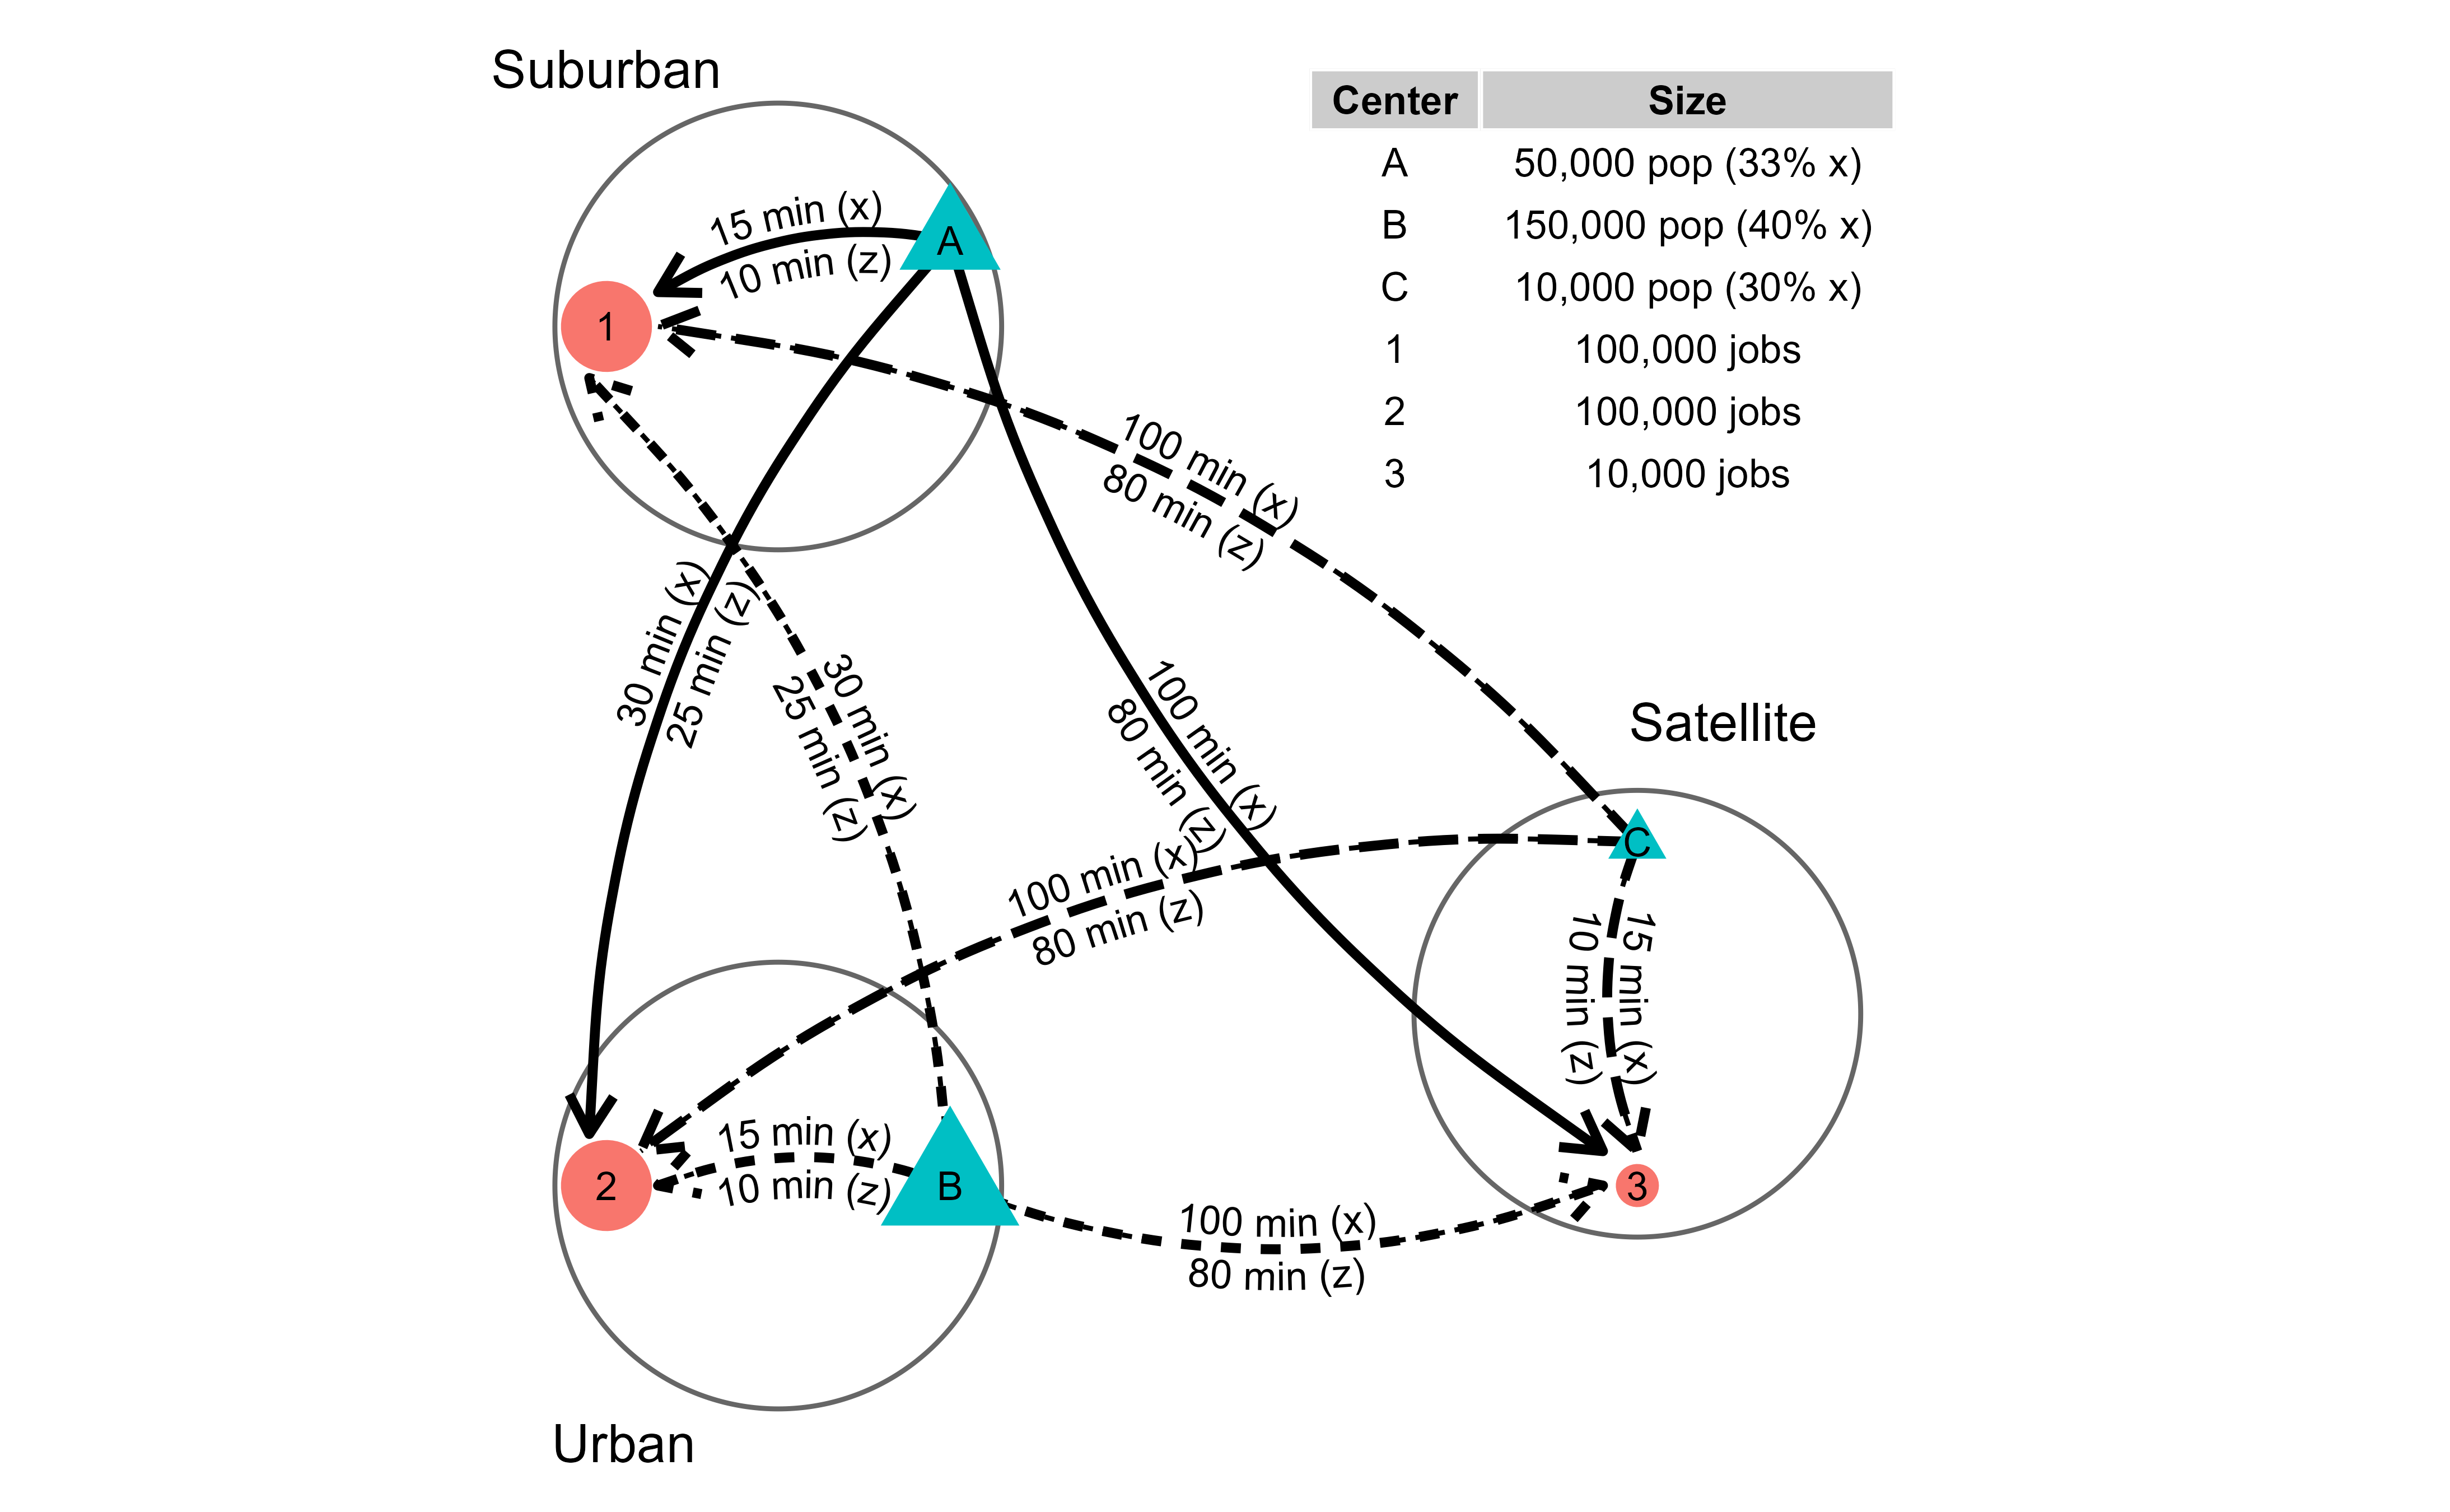
\includegraphics[width=0.85\linewidth]{images/Fig1} 

}

\caption{\label{fig:Fig1} Multimodal synthetic example: locations of employment centers (in orange), population centers (in blue), number of jobs and population, and travel times for two modes (slower mode x and faster mode z).}\label{fig:synthetic-example-plot}
\end{figure}

From the perspective of access to a \emph{finite} amount of
opportunities in the region (\(210,000\) jobs), the sub-population that
is most proximate to jobs (low cost to reach), furthest from large
populations (less competition), and uses the fastest mode \(z\) (greater
range) can potentially reach the largest number of opportunities. This
appears to be the sub-population at \(A\) using mode \(z\).
Sub-populations located in opposite conditions (i.e., more distant from
jobs, close to large populations, and using slower mode \(x\)) are at a
relative disadvantage. The competition for opportunities between
different mode-using populations matters as it reflects how well the
land-use and transport system serves (or does not serve) certain
populations.

\global\setlength{\Oldarrayrulewidth}{\arrayrulewidth}

\global\setlength{\Oldtabcolsep}{\tabcolsep}

\setlength{\tabcolsep}{0pt}

\renewcommand*{\arraystretch}{1.5}



\providecommand{\ascline}[3]{\noalign{\global\arrayrulewidth #1}\arrayrulecolor[HTML]{#2}\cline{#3}}

\begin{longtable}[c]{|p{0.88in}|p{0.41in}|p{1.05in}|p{0.58in}|p{1.05in}|p{0.58in}|p{1.05in}}

\caption{Accessibility\ values\ at\ each\ origin\ (i)\ per\ mode\ (m)\ (columns\ three\ to\ five)\ and\ aggregated\ per\ i\ (columns\ six\ and\ seven)\ for\ the\ synthetic\ example.}\\

\ascline{1.5pt}{666666}{1-7}

\multicolumn{1}{>{\raggedright}m{\dimexpr 0.88in+0\tabcolsep}}{\textcolor[HTML]{000000}{\fontsize{11}{11}\selectfont{i}}} & \multicolumn{1}{>{\raggedright}m{\dimexpr 0.41in+0\tabcolsep}}{\textcolor[HTML]{000000}{\fontsize{11}{11}\selectfont{m}}} & \multicolumn{1}{!{\color[HTML]{666666}\vrule width 1pt}>{\raggedleft}m{\dimexpr 1.05in+0\tabcolsep}}{\textcolor[HTML]{000000}{\fontsize{11}{11}\selectfont{S}}\textcolor[HTML]{000000}{\textsubscript{\fontsize{11}{11}\selectfont{i}}}\textcolor[HTML]{000000}{\textsuperscript{\fontsize{11}{11}\selectfont{m}}}} & \multicolumn{1}{>{\raggedleft}m{\dimexpr 0.58in+0\tabcolsep}}{\textcolor[HTML]{000000}{\fontsize{11}{11}\selectfont{a}}\textcolor[HTML]{000000}{\textsubscript{\fontsize{11}{11}\selectfont{i}}}\textcolor[HTML]{000000}{\textsuperscript{\fontsize{11}{11}\selectfont{m}}}} & \multicolumn{1}{>{\raggedleft}m{\dimexpr 1.05in+0\tabcolsep}}{\textcolor[HTML]{000000}{\fontsize{11}{11}\selectfont{V}}\textcolor[HTML]{000000}{\textsubscript{\fontsize{11}{11}\selectfont{i}}}\textcolor[HTML]{000000}{\textsuperscript{\fontsize{11}{11}\selectfont{m}}}} & \multicolumn{1}{!{\color[HTML]{666666}\vrule width 1pt}>{\raggedleft}m{\dimexpr 0.58in+0\tabcolsep}}{\textcolor[HTML]{000000}{\fontsize{11}{11}\selectfont{a}}\textcolor[HTML]{000000}{\textsubscript{\fontsize{11}{11}\selectfont{i}}}} & \multicolumn{1}{>{\raggedleft}m{\dimexpr 1.05in+0\tabcolsep}}{\textcolor[HTML]{000000}{\fontsize{11}{11}\selectfont{V}}\textcolor[HTML]{000000}{\textsubscript{\fontsize{11}{11}\selectfont{i}}}} \\

\ascline{1.5pt}{666666}{1-7}\endfirsthead \caption[]{Accessibility\ values\ at\ each\ origin\ (i)\ per\ mode\ (m)\ (columns\ three\ to\ five)\ and\ aggregated\ per\ i\ (columns\ six\ and\ seven)\ for\ the\ synthetic\ example.}\\

\ascline{1.5pt}{666666}{1-7}

\multicolumn{1}{>{\raggedright}m{\dimexpr 0.88in+0\tabcolsep}}{\textcolor[HTML]{000000}{\fontsize{11}{11}\selectfont{i}}} & \multicolumn{1}{>{\raggedright}m{\dimexpr 0.41in+0\tabcolsep}}{\textcolor[HTML]{000000}{\fontsize{11}{11}\selectfont{m}}} & \multicolumn{1}{!{\color[HTML]{666666}\vrule width 1pt}>{\raggedleft}m{\dimexpr 1.05in+0\tabcolsep}}{\textcolor[HTML]{000000}{\fontsize{11}{11}\selectfont{S}}\textcolor[HTML]{000000}{\textsubscript{\fontsize{11}{11}\selectfont{i}}}\textcolor[HTML]{000000}{\textsuperscript{\fontsize{11}{11}\selectfont{m}}}} & \multicolumn{1}{>{\raggedleft}m{\dimexpr 0.58in+0\tabcolsep}}{\textcolor[HTML]{000000}{\fontsize{11}{11}\selectfont{a}}\textcolor[HTML]{000000}{\textsubscript{\fontsize{11}{11}\selectfont{i}}}\textcolor[HTML]{000000}{\textsuperscript{\fontsize{11}{11}\selectfont{m}}}} & \multicolumn{1}{>{\raggedleft}m{\dimexpr 1.05in+0\tabcolsep}}{\textcolor[HTML]{000000}{\fontsize{11}{11}\selectfont{V}}\textcolor[HTML]{000000}{\textsubscript{\fontsize{11}{11}\selectfont{i}}}\textcolor[HTML]{000000}{\textsuperscript{\fontsize{11}{11}\selectfont{m}}}} & \multicolumn{1}{!{\color[HTML]{666666}\vrule width 1pt}>{\raggedleft}m{\dimexpr 0.58in+0\tabcolsep}}{\textcolor[HTML]{000000}{\fontsize{11}{11}\selectfont{a}}\textcolor[HTML]{000000}{\textsubscript{\fontsize{11}{11}\selectfont{i}}}} & \multicolumn{1}{>{\raggedleft}m{\dimexpr 1.05in+0\tabcolsep}}{\textcolor[HTML]{000000}{\fontsize{11}{11}\selectfont{V}}\textcolor[HTML]{000000}{\textsubscript{\fontsize{11}{11}\selectfont{i}}}} \\

\ascline{1.5pt}{666666}{1-7}\endhead



\multicolumn{1}{>{\raggedright}m{\dimexpr 0.88in+0\tabcolsep}}{} & \multicolumn{1}{>{\raggedright}m{\dimexpr 0.41in+0\tabcolsep}}{\textcolor[HTML]{000000}{\fontsize{11}{11}\selectfont{x}}} & \multicolumn{1}{!{\color[HTML]{666666}\vrule width 1pt}>{\raggedleft}m{\dimexpr 1.05in+0\tabcolsep}}{\textcolor[HTML]{000000}{\fontsize{11}{11}\selectfont{27,292.18}}} & \multicolumn{1}{>{\raggedleft}m{\dimexpr 0.58in+0\tabcolsep}}{\textcolor[HTML]{000000}{\fontsize{11}{11}\selectfont{0.95}}} & \multicolumn{1}{>{\raggedleft}m{\dimexpr 1.05in+0\tabcolsep}}{\textcolor[HTML]{000000}{\fontsize{11}{11}\selectfont{15,696.89}}} & \multicolumn{1}{!{\color[HTML]{666666}\vrule width 1pt}>{\raggedleft}m{\dimexpr 0.58in+0\tabcolsep}}{} & \multicolumn{1}{>{\raggedleft}m{\dimexpr 1.05in+0\tabcolsep}}{} \\





\multicolumn{1}{>{\raggedright}m{\dimexpr 0.88in+0\tabcolsep}}{\multirow[c]{-2}{*}{\parbox{0.88in}{\raggedright \textcolor[HTML]{000000}{\fontsize{11}{11}\selectfont{A}}}}} & \multicolumn{1}{>{\raggedright}m{\dimexpr 0.41in+0\tabcolsep}}{\textcolor[HTML]{000000}{\fontsize{11}{11}\selectfont{z}}} & \multicolumn{1}{!{\color[HTML]{666666}\vrule width 1pt}>{\raggedleft}m{\dimexpr 1.05in+0\tabcolsep}}{\textcolor[HTML]{000000}{\fontsize{11}{11}\selectfont{44,999.80}}} & \multicolumn{1}{>{\raggedleft}m{\dimexpr 0.58in+0\tabcolsep}}{\textcolor[HTML]{000000}{\fontsize{11}{11}\selectfont{1.57}}} & \multicolumn{1}{>{\raggedleft}m{\dimexpr 1.05in+0\tabcolsep}}{\textcolor[HTML]{000000}{\fontsize{11}{11}\selectfont{51,785.72}}} & \multicolumn{1}{!{\color[HTML]{666666}\vrule width 1pt}>{\raggedleft}m{\dimexpr 0.58in+0\tabcolsep}}{\multirow[c]{-2}{*}{\parbox{0.58in}{\raggedleft \textcolor[HTML]{000000}{\fontsize{11}{11}\selectfont{1.36}}}}} & \multicolumn{1}{>{\raggedleft}m{\dimexpr 1.05in+0\tabcolsep}}{\multirow[c]{-2}{*}{\parbox{1.05in}{\raggedleft \textcolor[HTML]{000000}{\fontsize{11}{11}\selectfont{67,482.61}}}}} \\

\ascline{1pt}{666666}{1-7}



\multicolumn{1}{>{\raggedright}m{\dimexpr 0.88in+0\tabcolsep}}{} & \multicolumn{1}{>{\raggedright}m{\dimexpr 0.41in+0\tabcolsep}}{\textcolor[HTML]{000000}{\fontsize{11}{11}\selectfont{x}}} & \multicolumn{1}{!{\color[HTML]{666666}\vrule width 1pt}>{\raggedleft}m{\dimexpr 1.05in+0\tabcolsep}}{\textcolor[HTML]{000000}{\fontsize{11}{11}\selectfont{27,292.18}}} & \multicolumn{1}{>{\raggedleft}m{\dimexpr 0.58in+0\tabcolsep}}{\textcolor[HTML]{000000}{\fontsize{11}{11}\selectfont{0.64}}} & \multicolumn{1}{>{\raggedleft}m{\dimexpr 1.05in+0\tabcolsep}}{\textcolor[HTML]{000000}{\fontsize{11}{11}\selectfont{38,170.03}}} & \multicolumn{1}{!{\color[HTML]{666666}\vrule width 1pt}>{\raggedleft}m{\dimexpr 0.58in+0\tabcolsep}}{} & \multicolumn{1}{>{\raggedleft}m{\dimexpr 1.05in+0\tabcolsep}}{} \\





\multicolumn{1}{>{\raggedright}m{\dimexpr 0.88in+0\tabcolsep}}{\multirow[c]{-2}{*}{\parbox{0.88in}{\raggedright \textcolor[HTML]{000000}{\fontsize{11}{11}\selectfont{B}}}}} & \multicolumn{1}{>{\raggedright}m{\dimexpr 0.41in+0\tabcolsep}}{\textcolor[HTML]{000000}{\fontsize{11}{11}\selectfont{z}}} & \multicolumn{1}{!{\color[HTML]{666666}\vrule width 1pt}>{\raggedleft}m{\dimexpr 1.05in+0\tabcolsep}}{\textcolor[HTML]{000000}{\fontsize{11}{11}\selectfont{44,999.80}}} & \multicolumn{1}{>{\raggedleft}m{\dimexpr 0.58in+0\tabcolsep}}{\textcolor[HTML]{000000}{\fontsize{11}{11}\selectfont{1.05}}} & \multicolumn{1}{>{\raggedleft}m{\dimexpr 1.05in+0\tabcolsep}}{\textcolor[HTML]{000000}{\fontsize{11}{11}\selectfont{94,468.91}}} & \multicolumn{1}{!{\color[HTML]{666666}\vrule width 1pt}>{\raggedleft}m{\dimexpr 0.58in+0\tabcolsep}}{\multirow[c]{-2}{*}{\parbox{0.58in}{\raggedleft \textcolor[HTML]{000000}{\fontsize{11}{11}\selectfont{0.88}}}}} & \multicolumn{1}{>{\raggedleft}m{\dimexpr 1.05in+0\tabcolsep}}{\multirow[c]{-2}{*}{\parbox{1.05in}{\raggedleft \textcolor[HTML]{000000}{\fontsize{11}{11}\selectfont{132,638.94}}}}} \\

\ascline{1pt}{666666}{1-7}



\multicolumn{1}{>{\raggedright}m{\dimexpr 0.88in+0\tabcolsep}}{} & \multicolumn{1}{>{\raggedright}m{\dimexpr 0.41in+0\tabcolsep}}{\textcolor[HTML]{000000}{\fontsize{11}{11}\selectfont{x}}} & \multicolumn{1}{!{\color[HTML]{666666}\vrule width 1pt}>{\raggedleft}m{\dimexpr 1.05in+0\tabcolsep}}{\textcolor[HTML]{000000}{\fontsize{11}{11}\selectfont{2,240.38}}} & \multicolumn{1}{>{\raggedleft}m{\dimexpr 0.58in+0\tabcolsep}}{\textcolor[HTML]{000000}{\fontsize{11}{11}\selectfont{0.68}}} & \multicolumn{1}{>{\raggedleft}m{\dimexpr 1.05in+0\tabcolsep}}{\textcolor[HTML]{000000}{\fontsize{11}{11}\selectfont{2,035.86}}} & \multicolumn{1}{!{\color[HTML]{666666}\vrule width 1pt}>{\raggedleft}m{\dimexpr 0.58in+0\tabcolsep}}{} & \multicolumn{1}{>{\raggedleft}m{\dimexpr 1.05in+0\tabcolsep}}{} \\





\multicolumn{1}{>{\raggedright}m{\dimexpr 0.88in+0\tabcolsep}}{\multirow[c]{-2}{*}{\parbox{0.88in}{\raggedright \textcolor[HTML]{000000}{\fontsize{11}{11}\selectfont{C}}}}} & \multicolumn{1}{>{\raggedright}m{\dimexpr 0.41in+0\tabcolsep}}{\textcolor[HTML]{000000}{\fontsize{11}{11}\selectfont{z}}} & \multicolumn{1}{!{\color[HTML]{666666}\vrule width 1pt}>{\raggedleft}m{\dimexpr 1.05in+0\tabcolsep}}{\textcolor[HTML]{000000}{\fontsize{11}{11}\selectfont{3,745.89}}} & \multicolumn{1}{>{\raggedleft}m{\dimexpr 0.58in+0\tabcolsep}}{\textcolor[HTML]{000000}{\fontsize{11}{11}\selectfont{1.12}}} & \multicolumn{1}{>{\raggedleft}m{\dimexpr 1.05in+0\tabcolsep}}{\textcolor[HTML]{000000}{\fontsize{11}{11}\selectfont{7,842.59}}} & \multicolumn{1}{!{\color[HTML]{666666}\vrule width 1pt}>{\raggedleft}m{\dimexpr 0.58in+0\tabcolsep}}{\multirow[c]{-2}{*}{\parbox{0.58in}{\raggedleft \textcolor[HTML]{000000}{\fontsize{11}{11}\selectfont{0.99}}}}} & \multicolumn{1}{>{\raggedleft}m{\dimexpr 1.05in+0\tabcolsep}}{\multirow[c]{-2}{*}{\parbox{1.05in}{\raggedleft \textcolor[HTML]{000000}{\fontsize{11}{11}\selectfont{9,878.45}}}}} \\

\ascline{1pt}{666666}{1-7}



\multicolumn{1}{>{\raggedright}m{\dimexpr 0.88in+0\tabcolsep}}{\textcolor[HTML]{000000}{\fontsize{11}{11}\selectfont{TOTALS}}} & \multicolumn{1}{>{\raggedright}m{\dimexpr 0.41in+0\tabcolsep}}{\textcolor[HTML]{000000}{\fontsize{11}{11}\selectfont{}}} & \multicolumn{1}{!{\color[HTML]{666666}\vrule width 1pt}>{\raggedleft}m{\dimexpr 1.05in+0\tabcolsep}}{\textcolor[HTML]{000000}{\fontsize{11}{11}\selectfont{150,570.22}}} & \multicolumn{1}{>{\raggedleft}m{\dimexpr 0.58in+0\tabcolsep}}{\textcolor[HTML]{000000}{\fontsize{11}{11}\selectfont{N/A}}} & \multicolumn{1}{>{\raggedleft}m{\dimexpr 1.05in+0\tabcolsep}}{\textcolor[HTML]{000000}{\fontsize{11}{11}\selectfont{210,000.00}}} & \multicolumn{1}{!{\color[HTML]{666666}\vrule width 1pt}>{\raggedleft}m{\dimexpr 0.58in+0\tabcolsep}}{\textcolor[HTML]{000000}{\fontsize{11}{11}\selectfont{N/A}}} & \multicolumn{1}{>{\raggedleft}m{\dimexpr 1.05in+0\tabcolsep}}{\textcolor[HTML]{000000}{\fontsize{11}{11}\selectfont{210,000.00}}} \\

\ascline{1.5pt}{666666}{1-7}



\end{longtable}



\arrayrulecolor[HTML]{000000}

\global\setlength{\arrayrulewidth}{\Oldarrayrulewidth}

\global\setlength{\tabcolsep}{\Oldtabcolsep}

\renewcommand*{\arraystretch}{1}

The values calculated for \(S_i^m\) (Hansen-type accessibility),
\(a_i^m\) (Shen-type accessibility), and \(V_i^m\) (spatial
availability) for each \(i\) and \(m\) are shown in the middle three
columns and are aggregated for each \(i\) in the final two columns in
Table 1 . As in the example in Shen {[}24{]}, we use a negative
exponential impedance function
\(f^m(c_{ij}^m) = \exp(-\beta\cdot c_{ij})\) with \(\beta=0.1\) for both
\(x\) and \(z\) modes for all accessibility measures calculations.
Notice that in this example we use the same impedance function but the
travel times are different for the two modes. More generally, it is
possible to use different impedance functions for the modes, as
demonstrated in the empirical example in the following section.

Hansen-type accessibility \(S_i^m\) is presented for each origin and
mode in the third column of Table 1 . For all \(i\), the travel by \(z\)
results in higher values of \(S_i^m\) than travel by \(x\). Lack of
competition, or alternatively the assumption of an inexhaustible
resource in the calculation of \(S_i^m\), lead to a curious result.
Since the populations in \(A\) and \(B\) have the same travel impedance
to employment centers \(1\), \(2\) and \(3\) (either 15, 30, or 100
minutes using \(x\) or 10, 25, or 80 minutes using \(z\)), their values
of \(S_i^m\) are the same for both \(A\) and \(B\). Furthermore, the
total sum of \(S_i^m\) in the region is equal to 150,570.2. This value
lacks an intuitive interpretation: it represents the weighted sum of
opportunities that may be reached within the region according to the
travel impedance (i.e., the travel behavior and the characteristics of
the modes) and does not usefully translate into any sort of benchmark.
To connect this example to the aforementioned literature, \(S_i^m\) is
calculated in the work of Tahmasbi et al. {[}34{]}; they contrast
differences in \(S_i^m\) values between modes in a relative and
comparative sense, but make no further interpretation of the \(S_i^m\)
values. More densely populated metropolitan regions will tend to have
more opportunities and hence large \(S_i^m\) values and less densely
regions, smaller values; how much of these differences may simply an
artifact of region density?

In the fourth and sixth columns in Table 1 the results for Shen-type
accessibility are reported: first for both origin and mode \(a_i^m\) as
well as aggregated by the weighted mean mode-population (
\(\sum_m \frac{P_i^m}{P_i}*a_i^m\) ) to represent a value for each
origin \(a_i\). Unlike \(S_i^m\), this measure does considers
\emph{competition}. For instance, the population travelling by \(x\)
from \(A\) and \(B\) do not have the same values of \(a_i^m\) as those
travelling by \(z\). In fact, \(A\) has the highest values \(a_i^m\) and
\(a_i\) values since this center has the lowest travel impedance to
opportunities (lower than at \(C\), \(A\) and \(B\) are equal) and faces
relatively low competition, not being close to a relatively large
population (lower than at \(B\)).

However, the calculations of \(a_i^m\) are not constrained: the total
sum of \(a_i^m\) or \(a_i\) is practically meaningless since it
represents a sum of ratios. For instance, the population travelling by
\(z\) from \(A\) has a value of 1.57 jobs per job-seeking population
compared to 0.95 for users of mode \(x\). What is the meaning of these
values? The difference between these modes is equal to 0.62, but 0.62 of
what? How many more job opportunities can users of \(z\) reach compared
to user of \(x\)? When \(a_i^m\) is aggregated to \(a_i\) as shown in
the sixth column, the values face similar interpretability issues. The
Shen-type measure is implemented in aforementioned work of Tao et al.
{[}47{]} to calculate modal \(a_i^m\) values and the aggregated \(a_i\)
is implemented in the work of Carpentier et al. {[}49{]}. However,
similar to Hansen-type accessibility, these works discuss relative and
spatially comparative differences in values, but veer from interpreting
the values of \(a_i^m\) or \(a_i\) themselves. In fairness,
interpretation is complicated by the multiple counting of opportunities
between zones and modes.

In contrast, spatial availability \(V_i\) considers competition and is
constrained such that the total sum of values is equal to the total
number of opportunities in the region (i.e., \(210,000\) jobs). Seen in
fifth column of Table 1 , the values of \(V_i^m\) in \(A\) and \(B\) are
not the same within each mode (as this measure considers competition).
In fact, at \(A\), users of mode \(z\) capture 36,088.84 more spatially
available jobs (of the \(210,000\) jobs in the region) than the
sub-population travelling by \(x\). The numerical difference is clear
since it refers to opportunities out of the total.

Furthermore, the proportional allocation mechanism also means that the
values of \(V_i^m\) for any origin \(i\) can be aggregated across \(m\)
and compared between zones (\(V_i = \sum_m{\sum_i{V_i^m}}\)). This
aggregation, \(V_i\), is shown in the seventh column in Table 1 . Again
looking at center \(A\), \(A\) is allocated 67,482.61 spatially
available opportunities for both modes. 77\% of this spatial
availability allocated to \(A\) is assigned to users of mode \(z\)
despite representing 66\% of \(A\)'s population.

Spatial availability can be further aggregated to better interpret
competition between modes. Across the entire region, 130,000 people use
\(z\) (62\% of the region population). However, users of \(z\) account
for 73\% of the region's total spatial availability - while the
remaining 27\% is allocated to users of mode \(x\) who are 38\%of the
total population. Notably, the population who uses \(x\) have 11\% fewer
spatially available opportunities than its share in the population. This
realization could lead us to ask normative questions: how unequal should
availability of opportunities be by mode? What intervention could help
to redistribute spatial availability to sub-populations commensurate
with their proportion of the total?

Since spatial availability is constrained and has an interpretable
meaning as a proportion of the total opportunities in the region, the
values at \(i\) have a straighforward interpretation. Inequality in
\(V_i^m\) values can be explored through a variety of approaches. For
instance, consider travel times. The population of travelers who use
\(z\) accounts for 67\% of the potential travel time traveled in the
region: this is 7\% less travel time than the proportion of spatial
available opportunities that is allocated to them. In other words, the
population of users of \(z\) travels fewer minutes overall and has more
spatial availability of opportunities than users of the slower mode
\(x\).

Alternatively, inequities in spatial availability between modes can be
explored through proportional benchmarks. A spatial availability per
capita \(v_i^m\) is presented in Equation (\ref{eq:SA-per-capita}):

\begin{equation}
\label{eq:SA-per-capita}
v_{i}^m = \frac{V_{i}^m}{P_{i}^m}
\end{equation}

The values of \(v_i^m\) for \(A\), \(B\), and \(C\) for users of \(x\)
are 0.95, 0.64 and 0.68 spatially available jobs per capita,
respectively. The values of \(v_i^m\) for users of \(z\) are much
higher, with values of: 1.57, 1.05 and 1.12 respectively. Users of
\(x\), especially those at \(B\) and \(C\), are directly impacted by the
jobs that are spatially available to users of \(z\) \emph{in addition
to} the mass effect (occurring at \(B\), high population density) and
high travel impedance (occurring at the Satellite \(C\)).

If, let us say, the planning goal was to have one spatially available
job per mode-using population, a policy intervention could be devised,
to reduce the values of \(v_i^z\) (making it slower or more expensive)
and increase he values of \(v_i^x\) (making it faster or les expensive).
The purpose of this synthetic demonstration is to show how spatial
availability can be used to quantify the competitive (dis)advantage in a
multimodal application. In what follows, we demonstrate the use of
multimodal spatial availability through an empirical example.

\hypertarget{empirical-example}{%
\section{Empirical example}\label{empirical-example}}

\hypertarget{context}{%
\subsection{Context}\label{context}}

The context for the empirical example is Madrid, Spain. This city
implemented a Low Emission Zone (LEZ) in 2017 to pursue goals set out in
the national climate change agenda, cut nitrogen dioxide levels, and to
prioritize people's movement in the city. LEZs elsewhere have similarly
been implemented as interventions to reduce GHG emissions, improve air
quality, and support sustainable mobility {[}50,51{]}. Though the rules
of exclusion vary by city, LEZs aim to deter/reduce traffic in
designated zones under threat of penalty (e.g., fines, seizure of
vehicle). In other words, LEZs implement a form of \emph{geographic
discrimination} as they change how people can reach opportunities by
making it more costly for some forms of travel, typically cars, to
circulate in predetermined zones. When considering opportunities as
finite in a region, this discrimination reduces the competition of one
mode and opens up opportunities for other modes to better thrive. At
their core, LEZs operate by changing the accessibility landscape of a
city from the perspective of multiple modes.

In geographic scope, the 2017 boundaries of the LEZ in Madrid were
relatively modest, covering only approximately 4.72
km\textsuperscript{2} of the central business district of the city (the
so-called LEZ Centro). As of this writing, there are plans to expand
these boundaries to the area inside the M-30, an orbital highway in
proximity to the city center (i.e., LEZ M-30). Within the 2017 LEZ
Centro implementation, all cars, motorcycles and freight vehicles with
environmental labels A or B (older makes and models of fossil fuel
internal combustion engine vehicles), were disallowed from entering the
zone unless they are used by residents or meet other exemptions. This
restriction impacted approximately half of all car trips that used to
travel into what is now the LEZ Centro {[}52{]}.

For this case study, we quantify spatial availability to opportunities
by different modes in Madrid. Particularly, we demonstrate how \(V_i^m\)
can be used to derive insights into how the restriction of car mobility
in areas around/within the LEZ Centro may have allowed more sustainable
(but often slower or more costly modes) to become more competitive.

\begin{figure}

{\centering 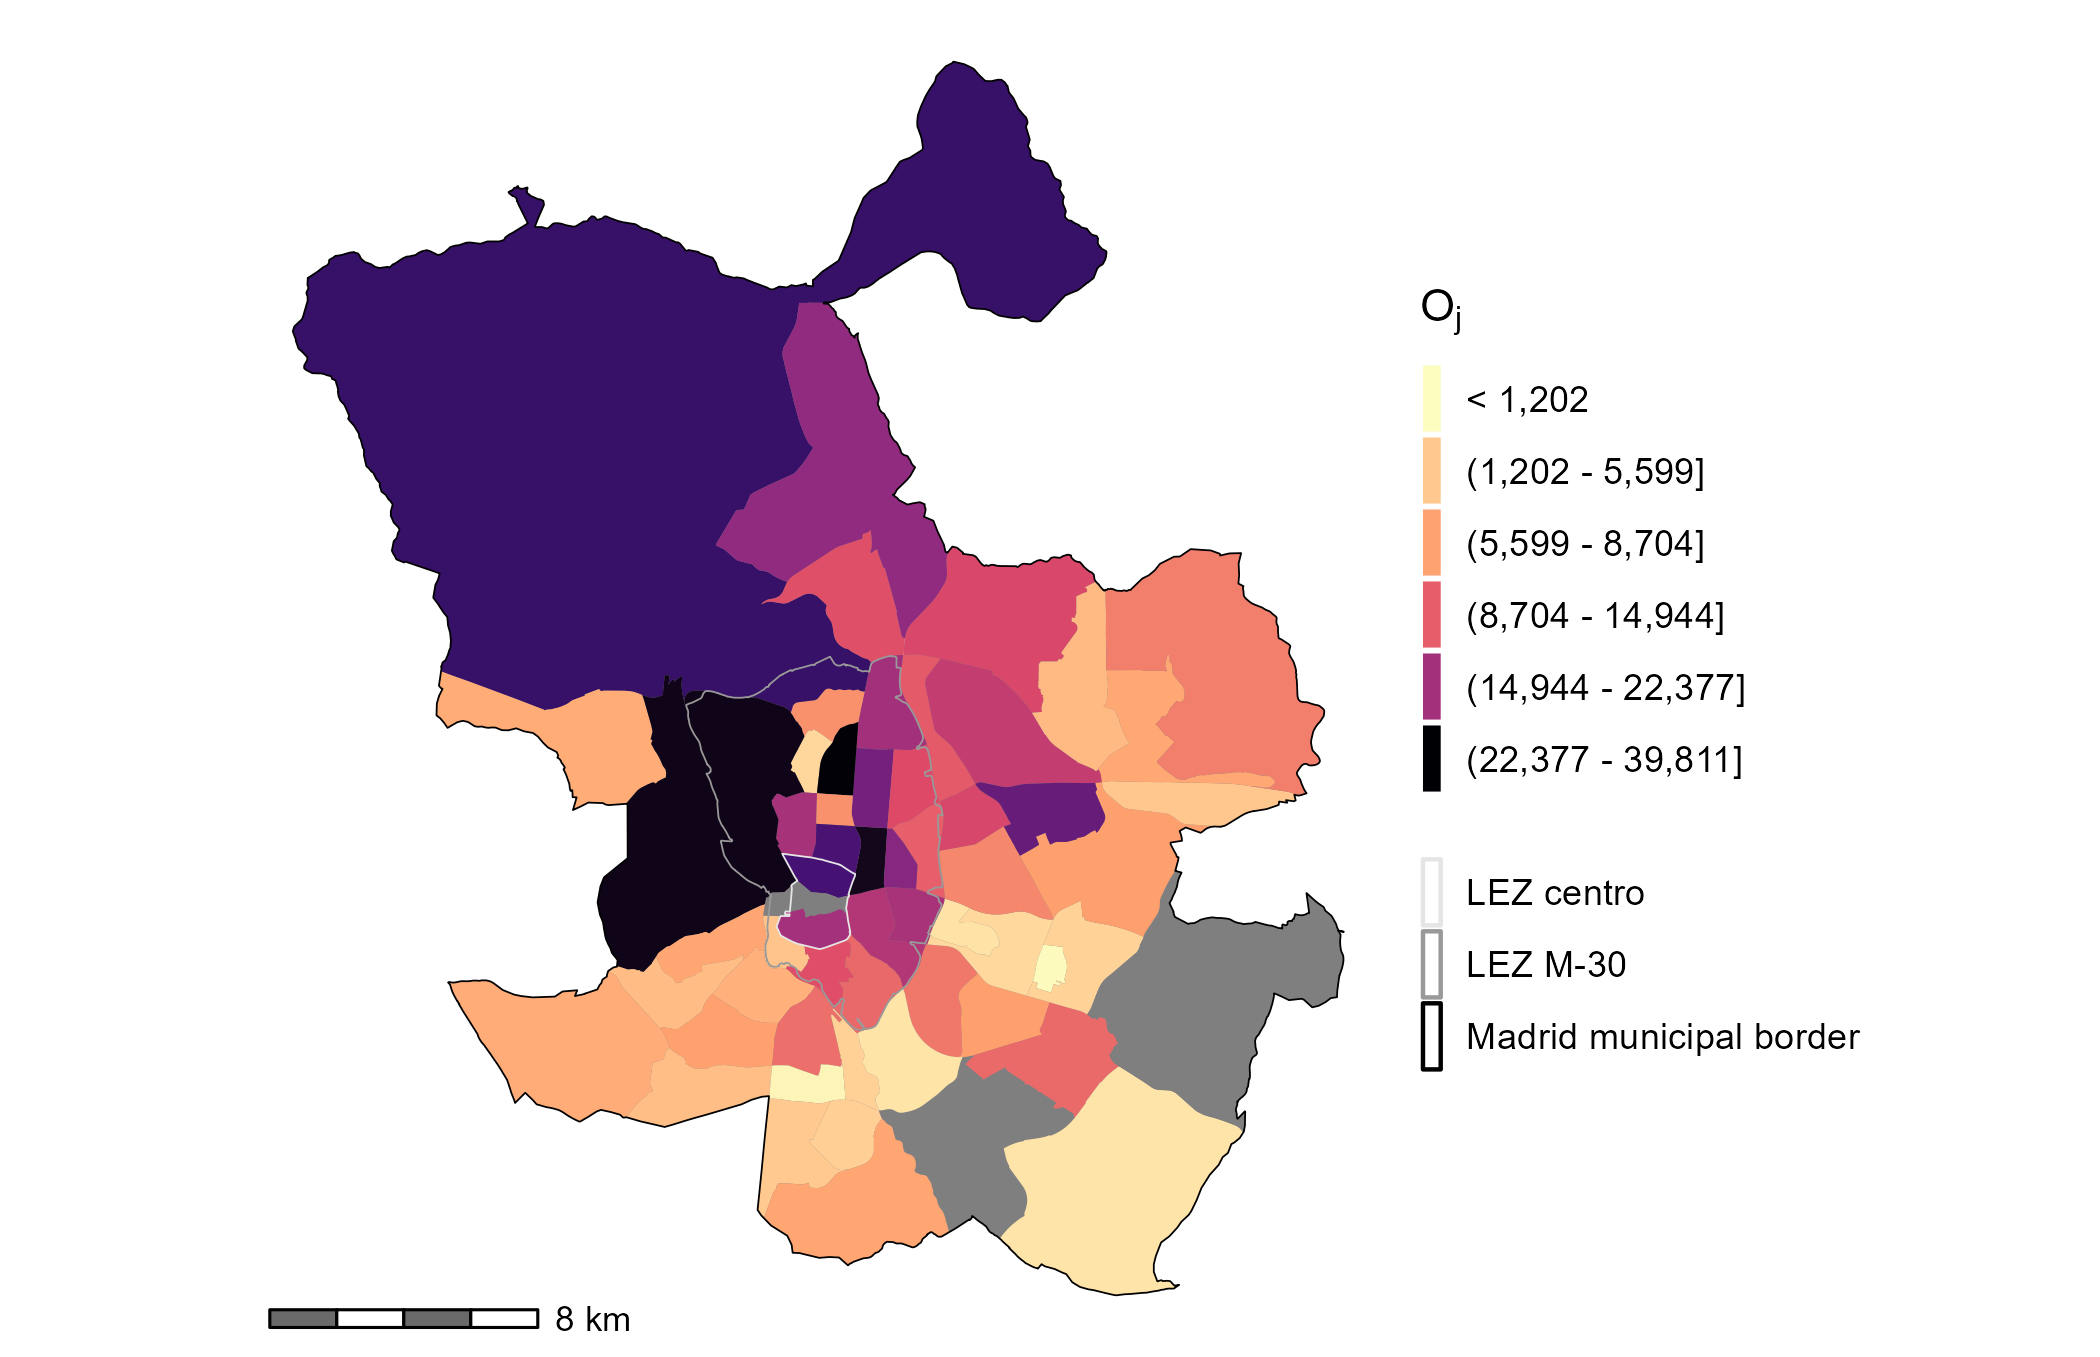
\includegraphics[width=0.85\linewidth]{images/Fig2} 

}

\caption{\label{fig:Fig2} Distribution of jobs taken by people living and working in Madrid as reported in the 2018 travel survey. Grey TAZs have no jobs. Ranges of values in the legend are quintiles. The TAZ shapefile is available from the Community of Madrid open data portal.}\label{fig:jobs-plot}
\end{figure}

\begin{figure}

{\centering 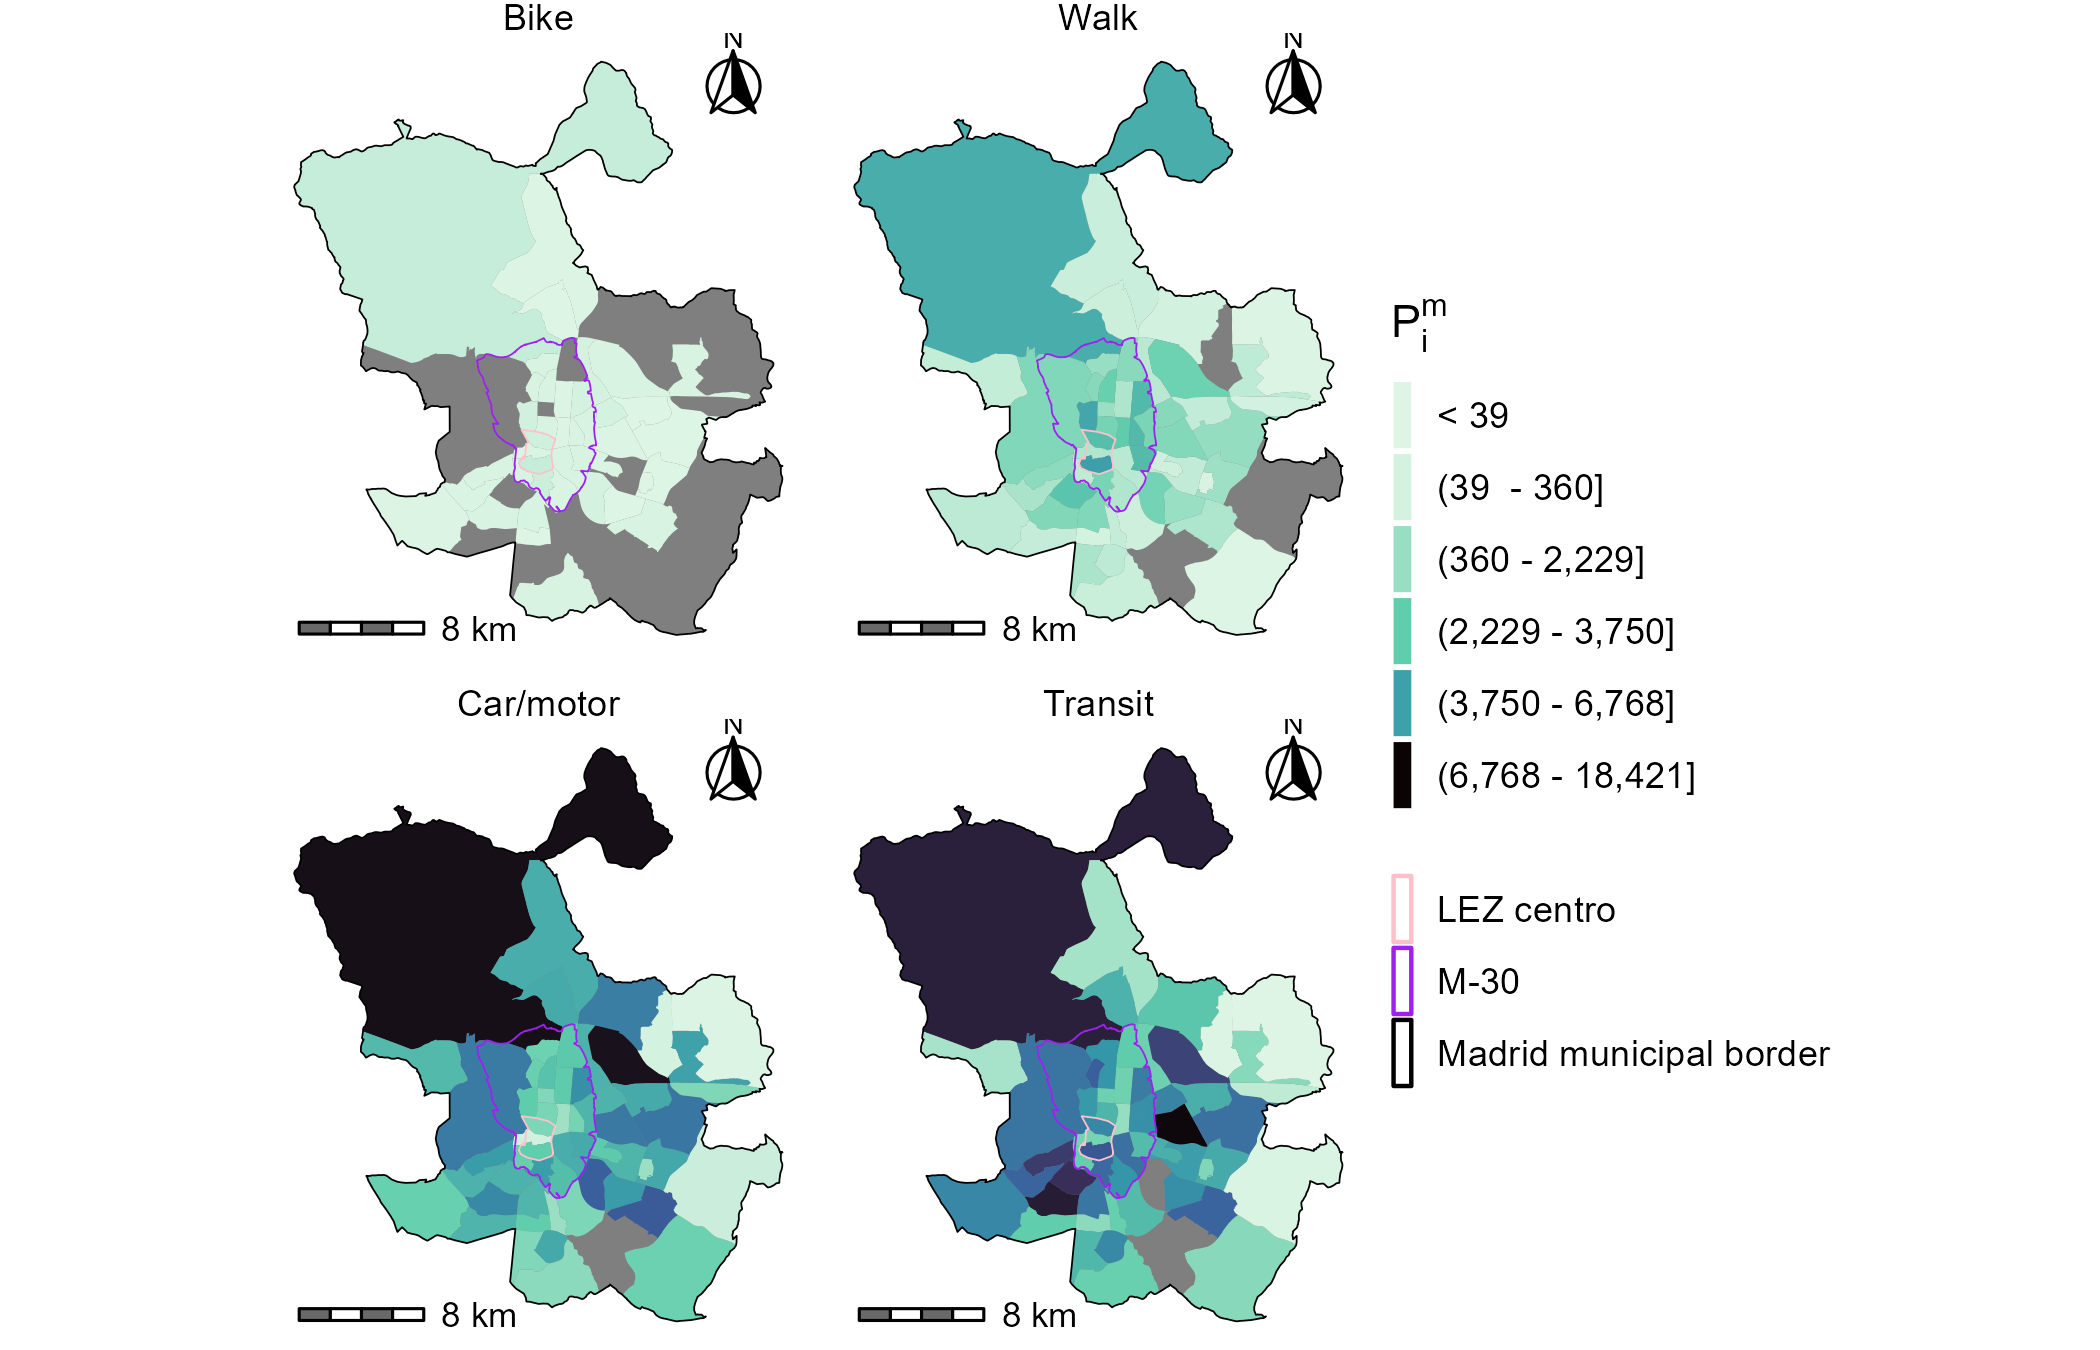
\includegraphics[width=0.85\linewidth]{images/Fig3} 

}

\caption{\label{fig:Fig3} Population living and working in Madrid by mode of transportation as reported in the 2018 travel survey and represented at the level of TAZ. Grey TAZ have no population. Ranges of values in the legend are quintiles. The TAZ shapefile is available from the Community of Madrid open data portal.}\label{fig:pop-plot}
\end{figure}

\hypertarget{data}{%
\subsection{Data}\label{data}}

The source of origin-destination data for our empirical example is the
2018 Travel Survey of the Community of Madrid {[}53{]}. This is a
representative survey that offers a snap-shot of travel patterns for a
typical weekday in 2018. The survey collected 222,744 trips from a
representative sample of 85,064 households across the traffic analysis
zones (TAZ) in the Community of Madrid. For context, the population
older than 3 years in the Community is 6,507,184.

In this example, we use all direct home-to-full-time-work trips, by all
modes. The trips are expanded using population weights. Figures
\ref{fig:Fig2} and \ref{fig:Fig3} show the number of workers and the
distribution of full-time jobs in the City of Madrid by TAZ. The TAZ
shapefiles are available from the Community of Madrid open data portal
{[}54{]}. The pink boundary represents the LEZ Centro in effect in 2017
and reflected in the 2018 travel survey. The purple boundary represents
the LEZ planned for the boundaries of the M-30 highway and is present in
the plots as a spatial reference for areas in proximity to the LEZ
Centro.

The total sum of jobs \(O_j\) are shown in Figure \ref{fig:Fig2} and the
populations that go to a work destination by four modal categories
\(P^m_i\), is displayed in Figure \ref{fig:Fig3}. The modal shares in
Figure \ref{fig:Fig3} are calculated based on the primary mode specified
in the survey and summarized into four categories as follows:

\begin{itemize}
\tightlist
\item
  Car/motor: all cars and operating modes (e.g., cab, private driver,
  company, rental car, main driver of a private car, passenger in a
  private car) and all public, private or company motorcycle/mopeds.
\item
  Transit: all bus, trams, and trains.
\item
  Bike: all bicycle trips (e.g., private, public, or company bike trips)
  and ``other'' types of micromobility options.
\item
  Walk: walking or by foot.
\end{itemize}

Some aggregation of modes is necessary to calculate the travel impedance
functions by mode. From Figure \ref{fig:Fig2}, it can be seen that the
largest concentration of jobs is within, near, and to the north of LEZ
Centro. The populations with access to those jobs by mode (Figure
\ref{fig:Fig3}) are spatially distinct. Travel by car and transit
represent 37\% and 47\% of the modal share respectively. The population
that travels by transit is more spatially distributed than those using
cars - particularly near and within LEZ Centro. This distribution is
likely caused by a variety of factors including: transit coverage and
service within with city, effective car infrastructure outside of the
M-30, and/or the impact of the LEZ Centro itself. From Figure
\ref{fig:Fig3}, it can be seen that active travel is less common than
motorised trips at 1\% and 15\% for cycling and walking respectively.
Noticeably, there is a positive trend between the walking and cycling in
zones where transit is also present. This positive trend is higher than
for car trip populations.

Travel times are provided within the travel survey by mode. This
information is used to calibrate mode-specific travel impedance
functions \(f^m(c_{ij}^m)\). To illustrate the modal differences in
travel times, the following descriptive statistics per mode are
presented:

\begin{itemize}
\tightlist
\item
  Car/motor: mean 36 minutes (min: 0 minutes, Q2: 15 minutes, Q3: 55
  minutes, max: 120 minutes)
\item
  Transit: mean 55 minutes (min: 1 minutes, Q2: 30 minutes, Q3: 80
  minutes, max: 120 minutes)
\item
  Bike: mean 34 minutes (min: 5 minutes, Q2: 15 minutes, Q3: 40 minutes,
  max: 115 minutes)
\item
  Walk: mean 27 minutes (min: 1 minutes, Q2: 10 minutes, Q3: 45 minutes,
  max: 119 minutes)
\end{itemize}

Impedance functions \(f^m(c_{ij}^m)\) are calibrated from the travel
times in the survey via the empirical trip length distribution (TLD). An
empirical TLD is given by the proportion of trips at various travel cost
bins. This distribution is then used to estimate the parameters of a
function for the travel impedance {[}as done in 55,56,57{]}. To fit the
impedance functions, we use the Maximum likelihood estimation and the
Nelder-Mead method for direct optimization available within the R
\{fitdistrplus\} package {[}58{]}. Based on goodness-of-fit criteria and
associated diagnostics, the gamma and log-normal probability density
functions are selected as best fitting curves for the motorised and
non-motorised modes respectively. The selection of functional forms
aligns with empirical examples in other regions {[}15,59,60{]}. The
shape and rate parameters for the gamma functions (motorised modes) are
1.8651852 and 0.051468 for car/motor and 2.7566235 and 0.0499193 for
transit; for the log-normal functions (non-motorised modes), the mean
and standard deviation parameters are 3.2372212 and 0.7575986 for bike
and 2.9918042 and 0.7575986 for walk.

Figure \ref{fig:Fig4} includes four plots to visualize the calibrated
impedance functions (represented as black lines) superimposed on the
empirical TLD. The impedance functions can be interpreted as the
propensity to travel (y-axis) given a trip travel time (x-axis). The
functions reflect a combination of possibilities and preferences: the
travel behavior given the transportation technologies available. For
example, trips shorter than 5 minutes do not occur frequently for any
mode; this reflects the spatial separation between places of residence
and places of work commonly seen in many cities. In terms of the
non-motorised modes, there is a preference towards walking trips around
15 minutes in duration, as seen from the highest value of
\(f^{walk}(c_{ij}^{walk})\). With respect to travel by bicycle, longer
travel times are more common; although the highest value of the
impedance also corresponds to approximately 15 minutes, the curve has a
longer tail and values decrease less rapidly at longer travel times than
is the case of \(f^{walk}(c_{ij}^{walk})\). A similar trend can be
observed for the motorised modal options where transit mode is more
spread out than car/motor mode. All in all, these functions represent
the propensity of travel by mode by duration of trip, and are used to
calculate the proportional allocation factors \(F_{ij}^m\) for
\(V_i^m\).

\begin{figure}

{\centering 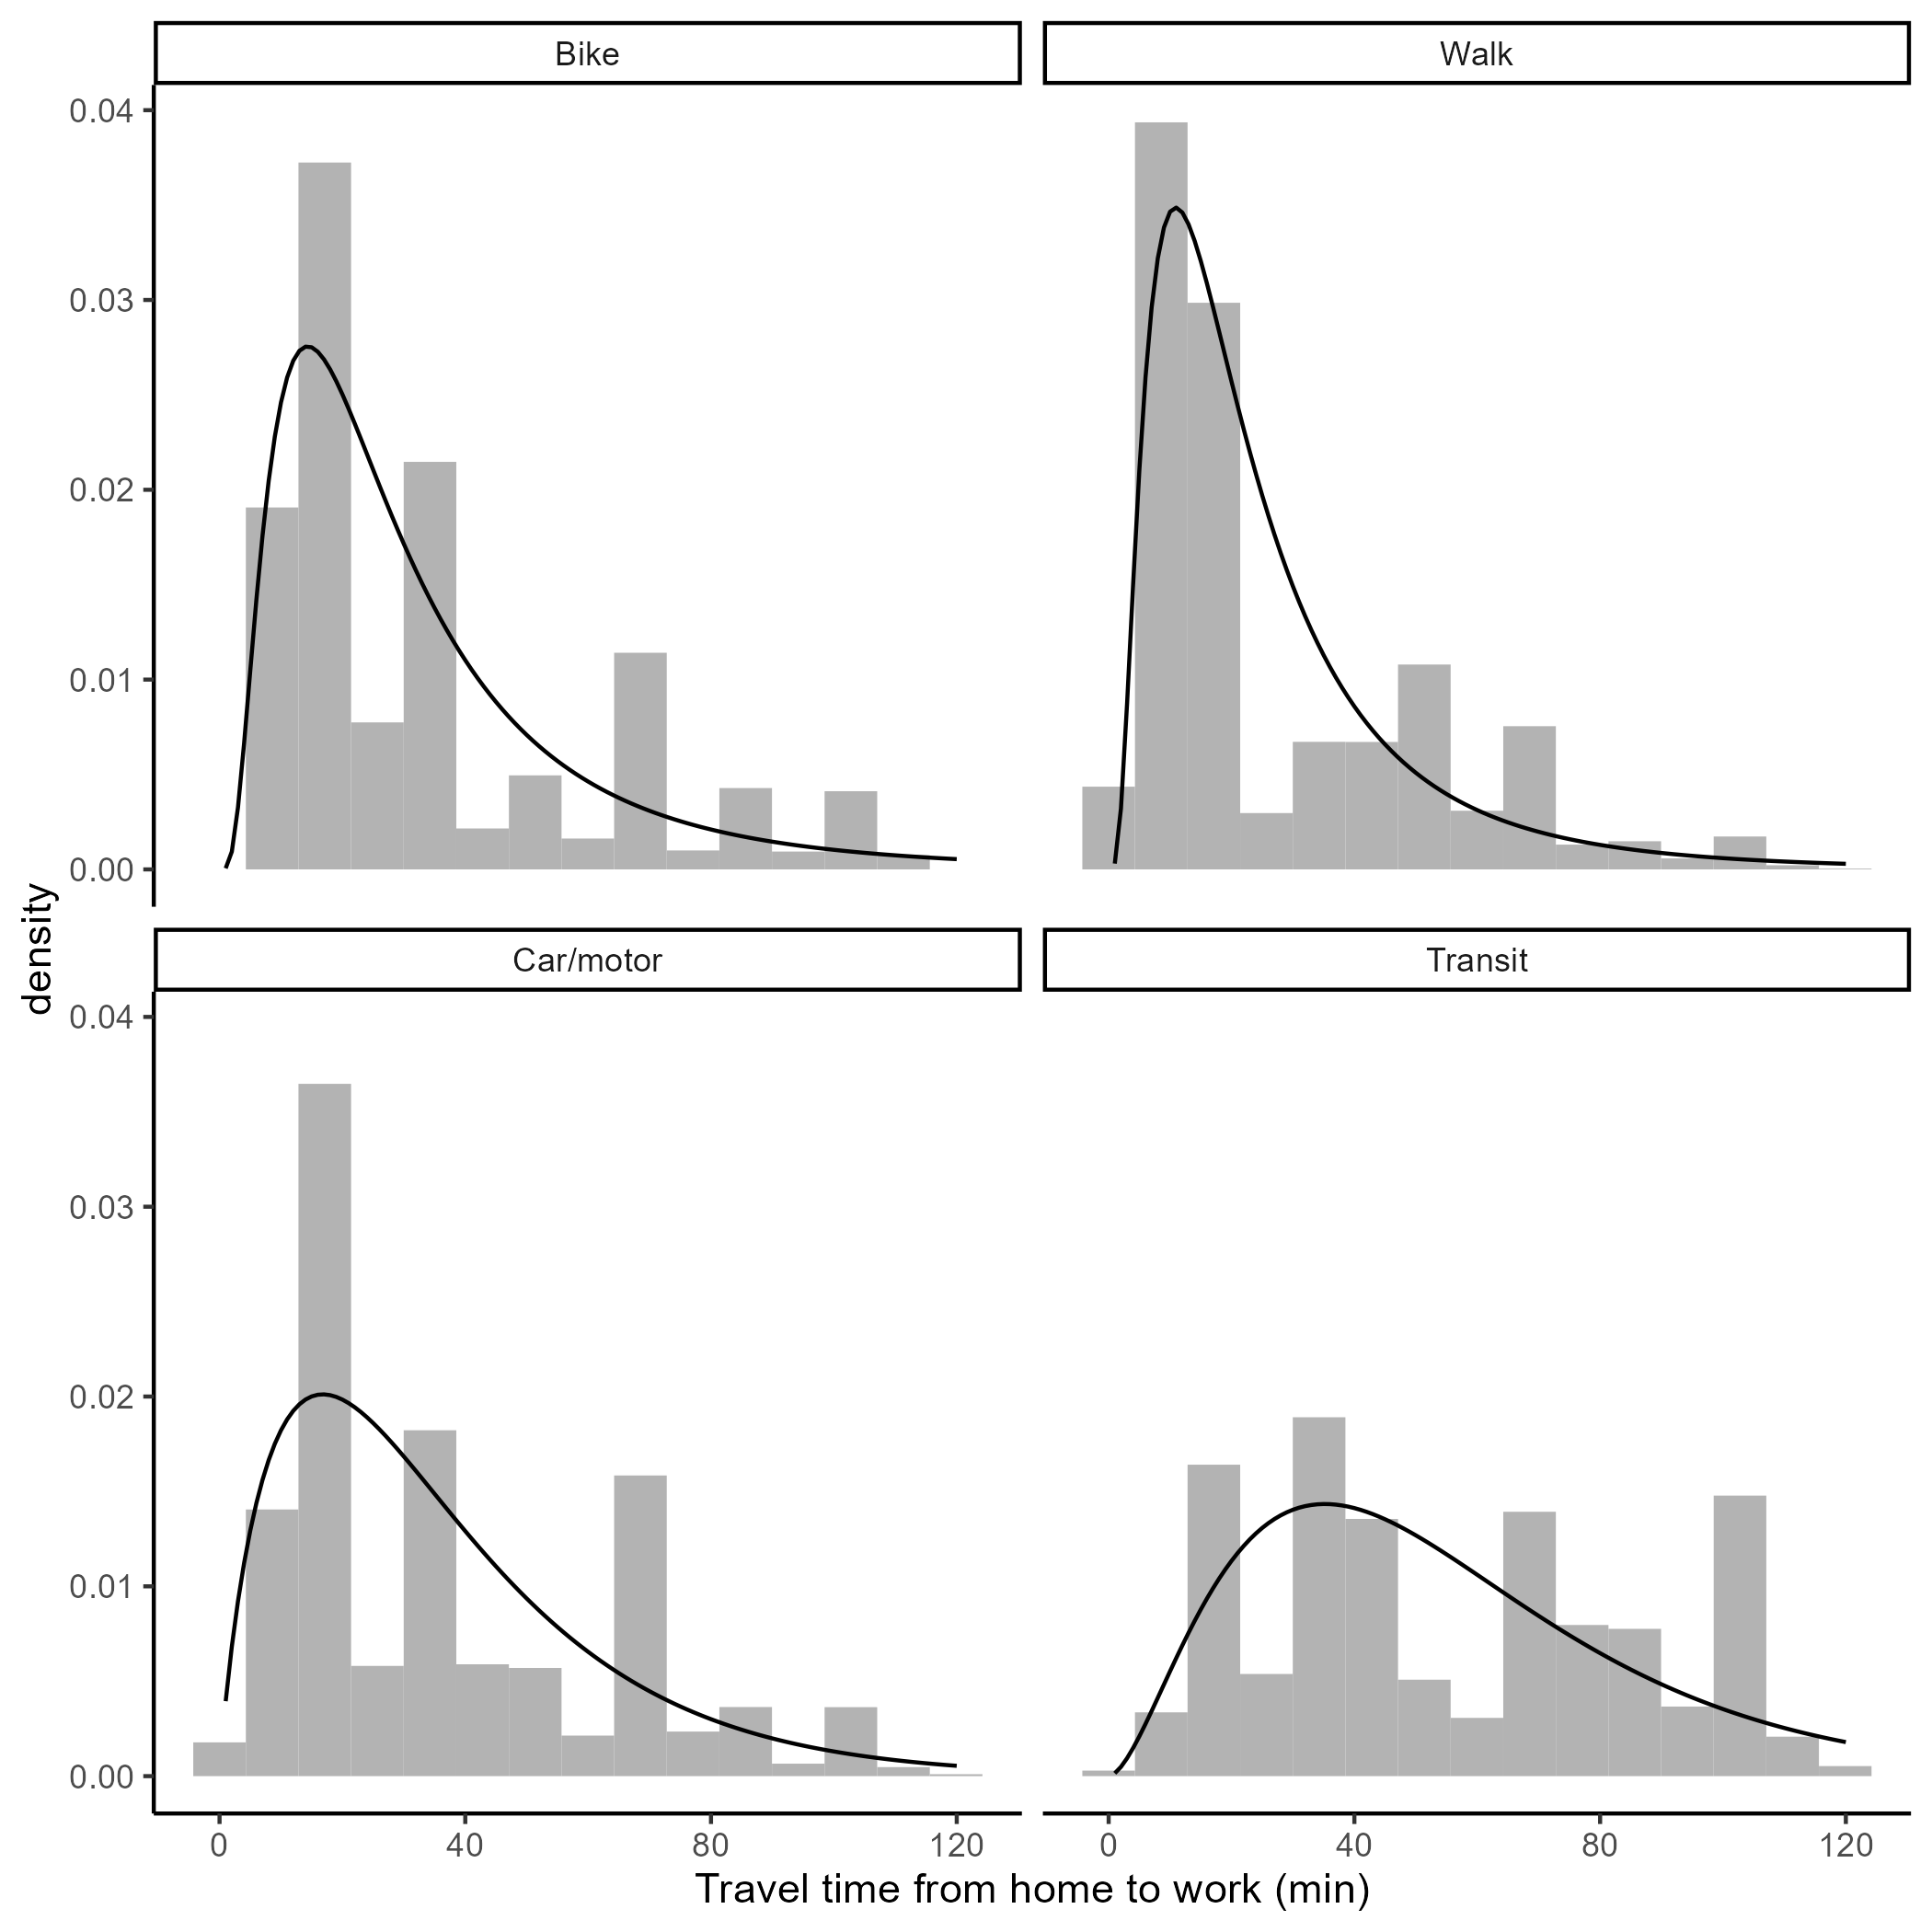
\includegraphics[width=0.85\linewidth]{images/Fig4} 

}

\caption{\label{fig:Fig4} Fitted impedance function against empirical TLD (bars) corresponding to the home to full-time work origin destination flows for the City of Madrid from the 2018 travel survey.}\label{fig:tlds-curves-m-plot}
\end{figure}

\hypertarget{results}{%
\subsection{Results}\label{results}}

It is worthwhile reiterating that the empirical example is a snapshot of
spatial availability by mode using modal home-work origin-destination
data from the 2018 travel survey. It reflects the travel behaviour after
LEZ implementation, i.e.~very few motorists commute into the LEZ centro.
Our purpose in this empirical example is to investigate the trends in
spatial availability of employment opportunities by mode, and illustrate
how spatial availability can be used to discuss modal competitive
advantage. We also discuss how multimodal spatial availability landscape
displayed in the Figure \ref{fig:Fig5} may have been impacted by the
LEZ.

\begin{figure}

{\centering 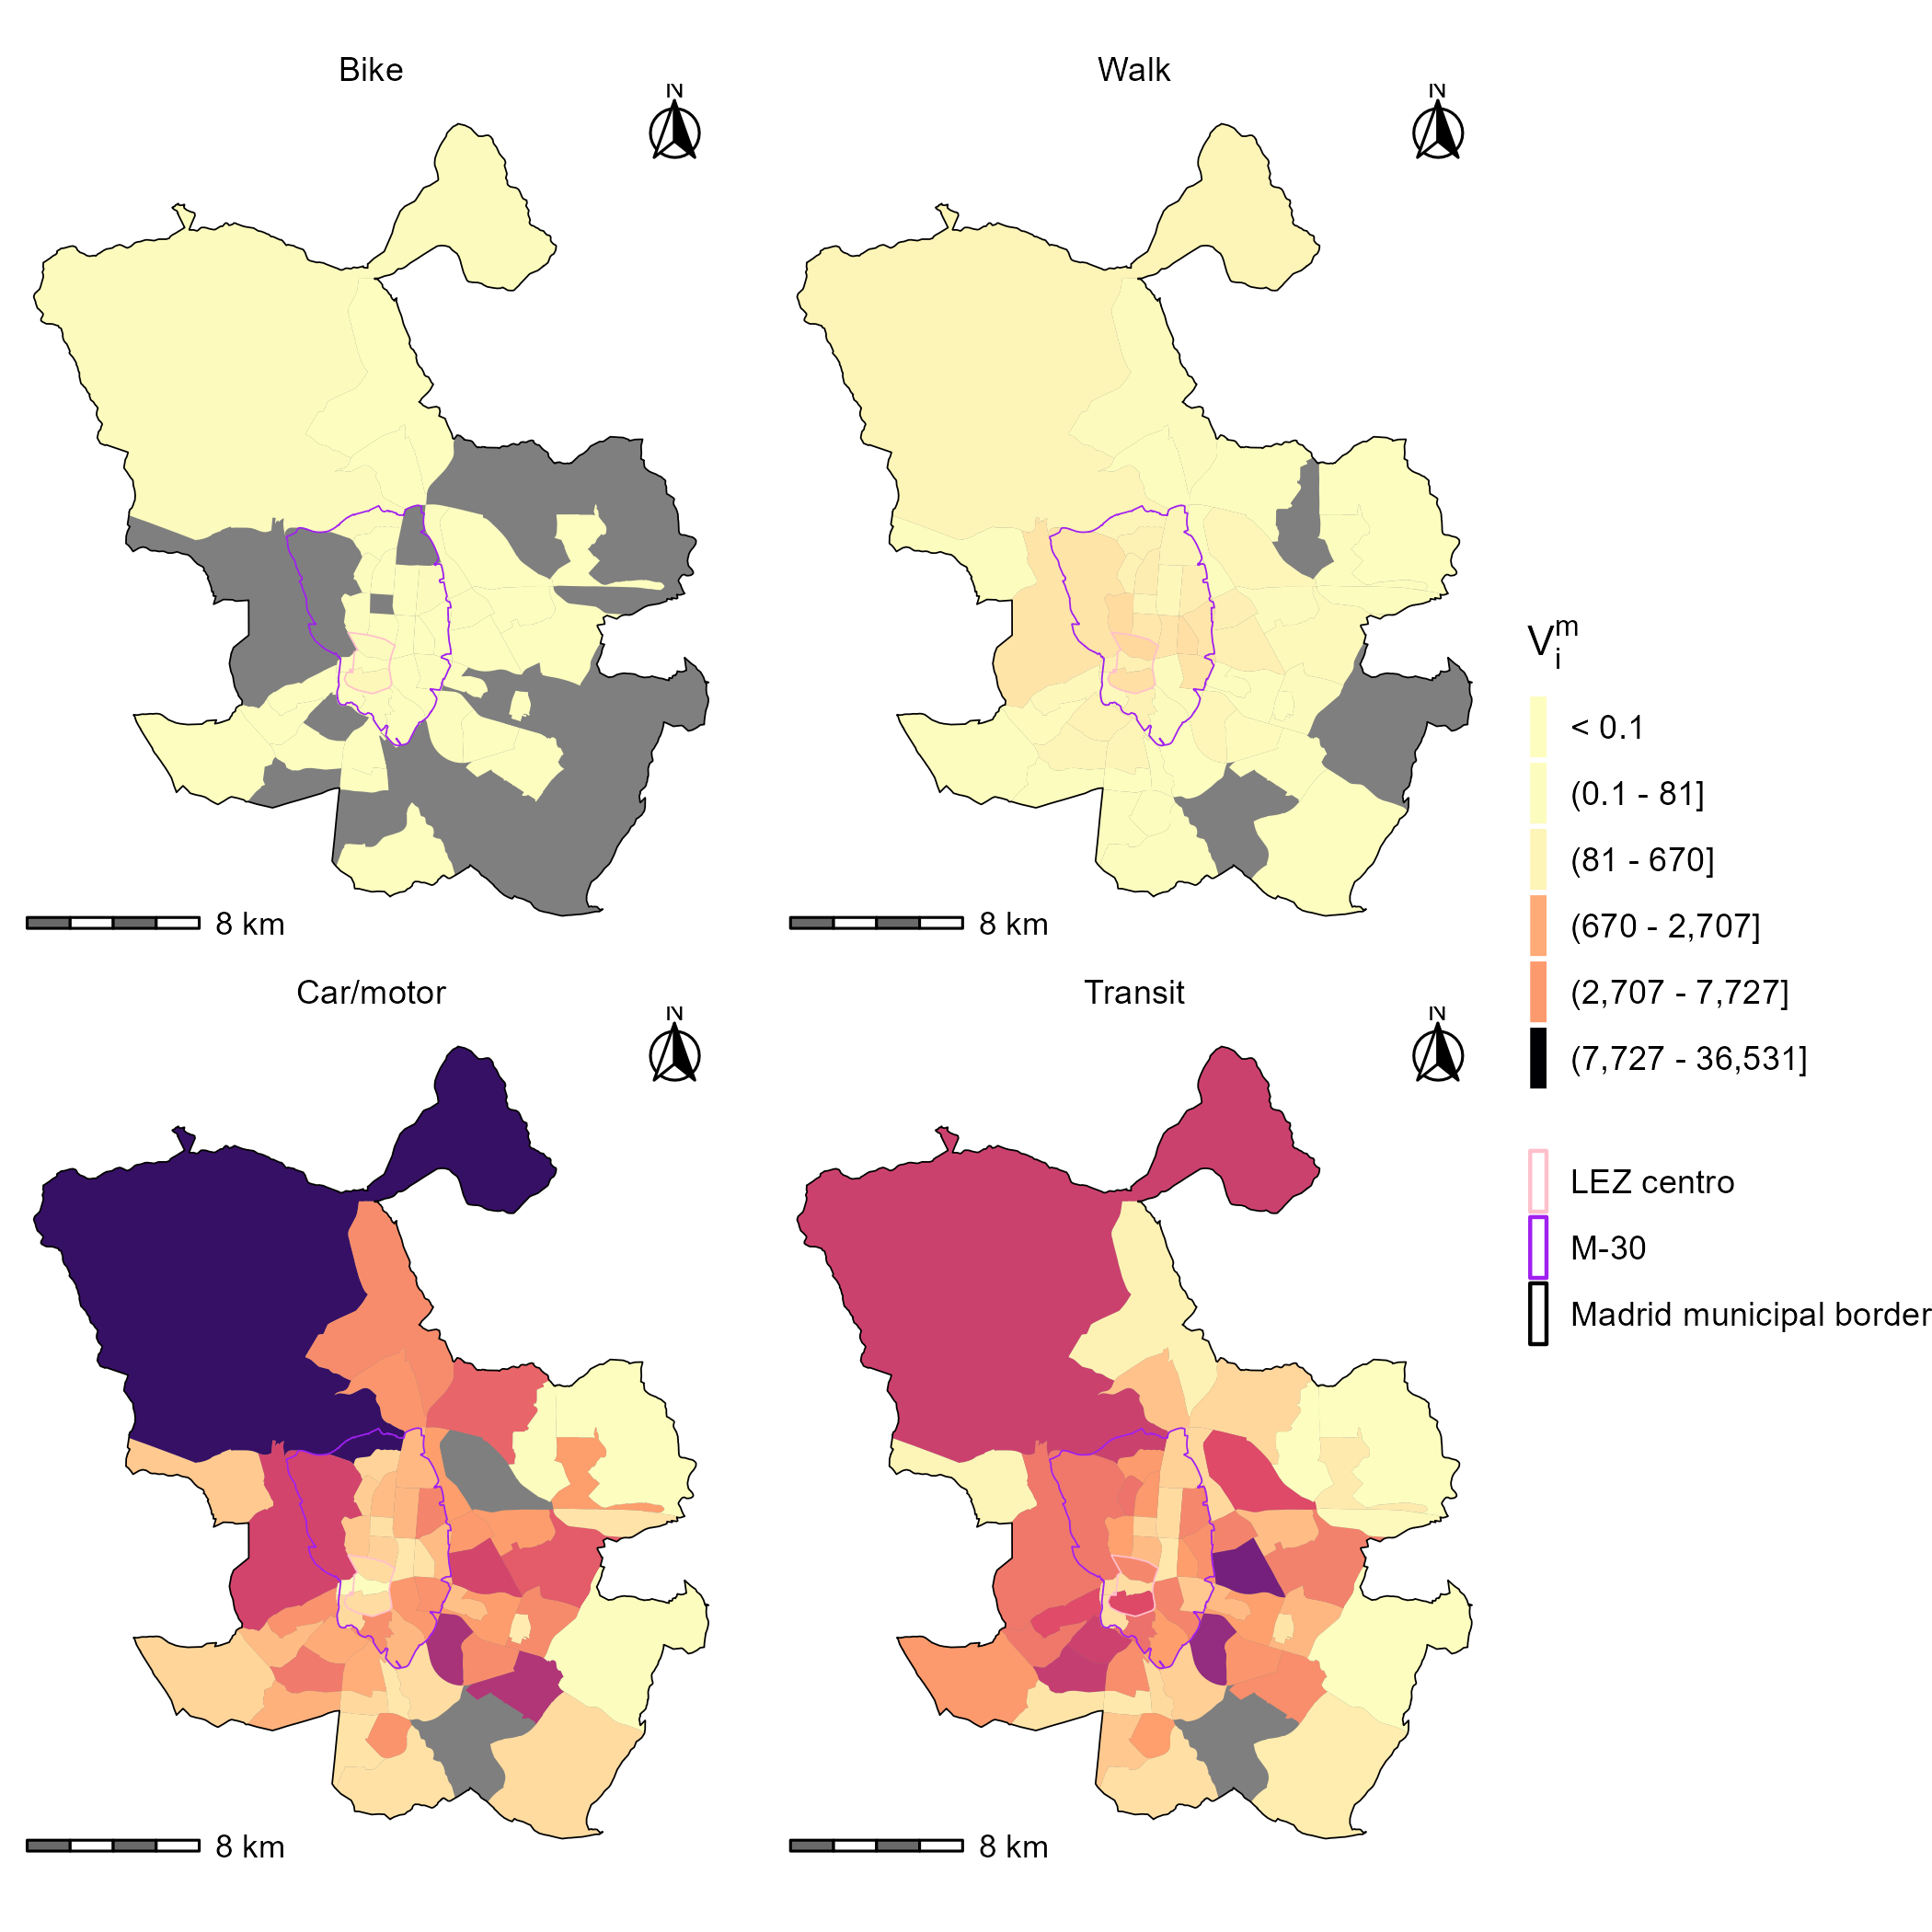
\includegraphics[width=0.85\linewidth]{images/Fig5} 

}

\caption{\label{fig:Fig5} Spatial availability of jobs per origin and mode $V_i^m$ in Madrid at the level of TAZ. Grey TAZ have no population. Ranges of values in the legend are quintiles. The TAZ shapefile is available from the Community of Madrid open data portal.}\label{fig:SA-m-plot}
\end{figure}

In Figure \ref{fig:Fig5}, the spatial availability of jobs \(V_i^m\) is
calculated for each of the four modes \(m\) at the level of traffic
analysis zones \(i\) in Madrid. \(V_i^m\) is a proportion of the total
number of 847,574 jobs in the region. Since \(V_i^m\) is calculated
based on the population of workers and the distribution of jobs, the
values can be understood as the number of full-time jobs that are
spatially available to full-time workers at that \(i\) traveling by mode
\(m\), relative to all the jobs in the city. This implementation of
spatial availability assumes that all employment opportunities are of
interest to the entire population but are proportional allocated based
on relative travel cost (informed by observed modal origin-destination
travel behaviour) and the relative amount of the mode-using population
residing in the zones.

There are noticeable differences in the magnitude of \(V_i^m\) between
modes in Figure \ref{fig:Fig5}. The majority of \(V_i^m\) (which is to
say of spatially available jobs) are allocated to workers travelling by
car and transit. In a way, this is to be expected since users of these
modes represent 84.1\% of the total population. However, the ability to
travel at greater speeds also impacts these results. Furthermore,
differences in \(V_i^m\) values within modes also exist in space: car
users outside of the M-30 region appear to enjoy greater spatial
availability, while some zones inside the M-30 have greater spatial
availability for transit. Overall, the magnitude of \(V_i^m\) values for
cyclists and pedestrians are lower than for car and transit but the
highest values of \(V_i^{bike}\) and \(V_i^{walk}\) tend to be found in
zones within the M-30 and origins with higher spatial availability by
transit.

The differences between the shares of modes and their shares of
spatially available opportunities highlights the competitive advantage
of certain modes, although this effect is not geographically uniform. As
seen in the left-most columns of Figure \ref{fig:Fig6}, users of
`car/motor' and `transit' together can avail 95.3\% of all jobs in the
city (Spatial Availability by Mode). However, car/motor users have a
disproportionate share of \(V_i^m\) relative to the population of users
of this mode (Population by Mode), compared to opportunities that are
spatially available to transit users. The combined population of car and
transit users is 36.6\% and 47.5\% respectively, but these populations
are allocated 48.0\% and 47.3\% respectively, of the city's jobs. When
treating the number of opportunities that can be reached as a finite
value (total: 847,574 opportunities), fewer opportunities are spatially
available to slower modes (i.e., walking and cycling), even taking into
account that their share is smaller overall. These modes are at a
disadvantage as a result of: the travel impedance for longer trips (see
Figure \ref{fig:Fig4}; their low population values values overall; and
larger populations in origins with high shares of travel by motorised
modes. These factors all contribute to the the car/motor mode being most
advantaged in capturing spatially available job opportunities overall.

\begin{figure}

{\centering 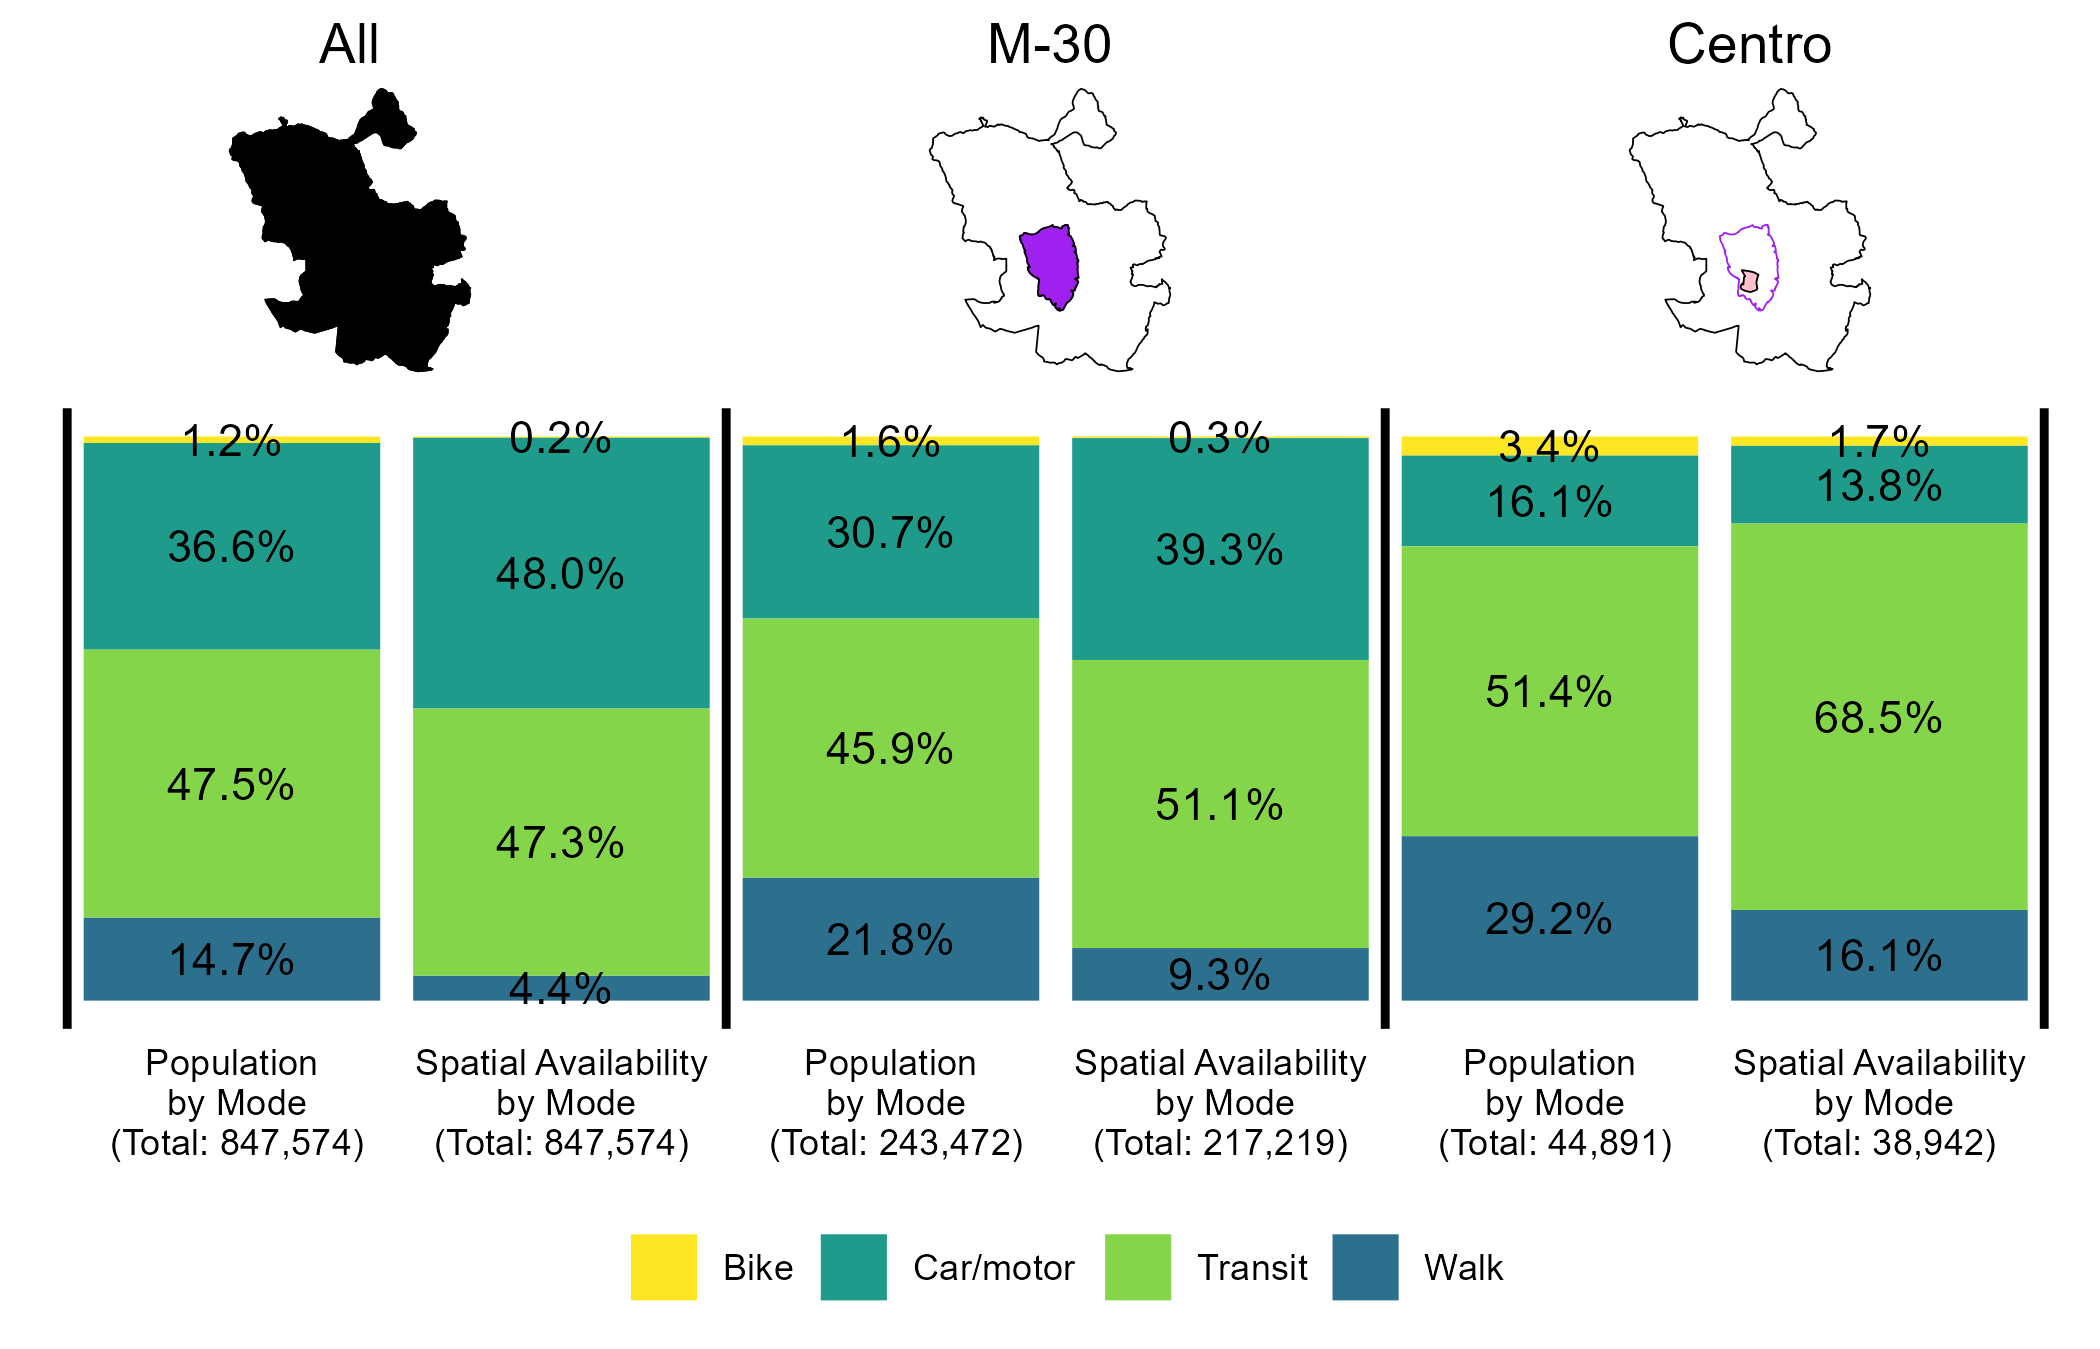
\includegraphics[width=0.85\linewidth]{images/Fig6} 

}

\caption{\label{fig:Fig6} Proportion of population by mode and spatial availability of jobs by mode aggregated for three areas. From left to right, the city of Madrid (All), the area within the M-30 highway (M-30), the area within the Centro region (Centro).}\label{fig:modal-V-comps-plot}
\end{figure}

The big picture demonstrates how, from the 2018 travel survey, car is
the most advantageous mode. However, it is interesting to notice that
this advantage appears to be blunted by the LEZ. Unlike the results for
the whole city and even within the M-30 ring, the proportion of car
users in Centro is larger than the proportion of opportunities spatially
available to them. The restriction on cars in effect reduces competition
by this mode, and leads to a relative increment of the mass effect of
the modes allowed within the LEZ, which also contains a large number of
jobs (see Figure \ref{fig:Fig2}). As summarized in the two right-most
columns in Figure \ref{fig:Fig6}, the proportion of jobs spatially
available to car in Centro is (13.8\% or 5,373 opportunities). For
reference, this is less than the proportion of the car users in Centro
(16.1\%), evidently less then the proportion of car users in the city,
and is the opposite of the overall trend (left-most columns) and within
the M-30 (middle columns).

It is also clear that more opportunities are spatially available to
non-car users within Centro. In the case of active travel, the
proportions of cyclists and walkers within LEZ Centro still exceeds the
proportions of jobs spatially available to them. Notably, this disparity
is drastically reduced compared to the rest of the city. As seen in
Figure \ref{fig:Fig6}, there is a higher proportion of opportunities
that are spatially available to pedestrians and cyclists in Centro than
in the City overall and in areas within the M-30. Within Centro, 1.7\%
and 16.1\% of opportunities are spatially available to bike and walk
modes respectively, while their populations represent 1.2\% and 14.7\%
of the population. By restricting the ability of cars to enter Centro,
the LEZ seems to contribute to leveling the playing field for slower
modes, in particular cycling and walking, but also transit. As seen in
the Figure \ref{fig:Fig6}, transit users are generally close to parity
across the region, with nearly as many spatially available jobs as
transit users. Still, this mode has the greatest advantage in LEZ Centro
with 68.5\% of spatially available jobs in Centro for 51.4\% of transit
users in Centro. This result makes intuitive sense: after car, it is the
mode with the greatest range, and unlike car it is unrestricted in the
LEZ Centro.

The spatial differences in the competitive (dis)advantage of spatial
availability between modes can also be visualized at a finer level of
granularity. Figure \ref{fig:Fig7} shows \(v_i^m\), the spatial
availability \(V_i^m\) divided by the population of users of \(m\).
Values of \(v_i^m\) below one are shown in shades of orange, and
indicate TAZs with less than one spatially available opportunity per
capita for the mode. Values above one are shown in shades of green, and
indicate TAZs with more than one spatially available opportunity per
capita for the mode. The highest spatial availability per capita (shown
in blue) is for car users in a zone northeast just beyond the M-30.
These plots illustrate in unambiguous fashion, and in a quantity that is
comparable over space and time, the advantage in terms of spatial
availability of car for most of the city (bottom left plot, areas
denoted with green \(v_i^m\) values above one). It can also be observed
that spatial availability of jobs is relatively well balanced for
transit users over most of the regions (i.e., many zones are light
orange or light green). Spatial availability of jobs for non-motorised
modes, in contrast, is low (under one) overall, although less so within
LEZ Centro.

\begin{figure}

{\centering 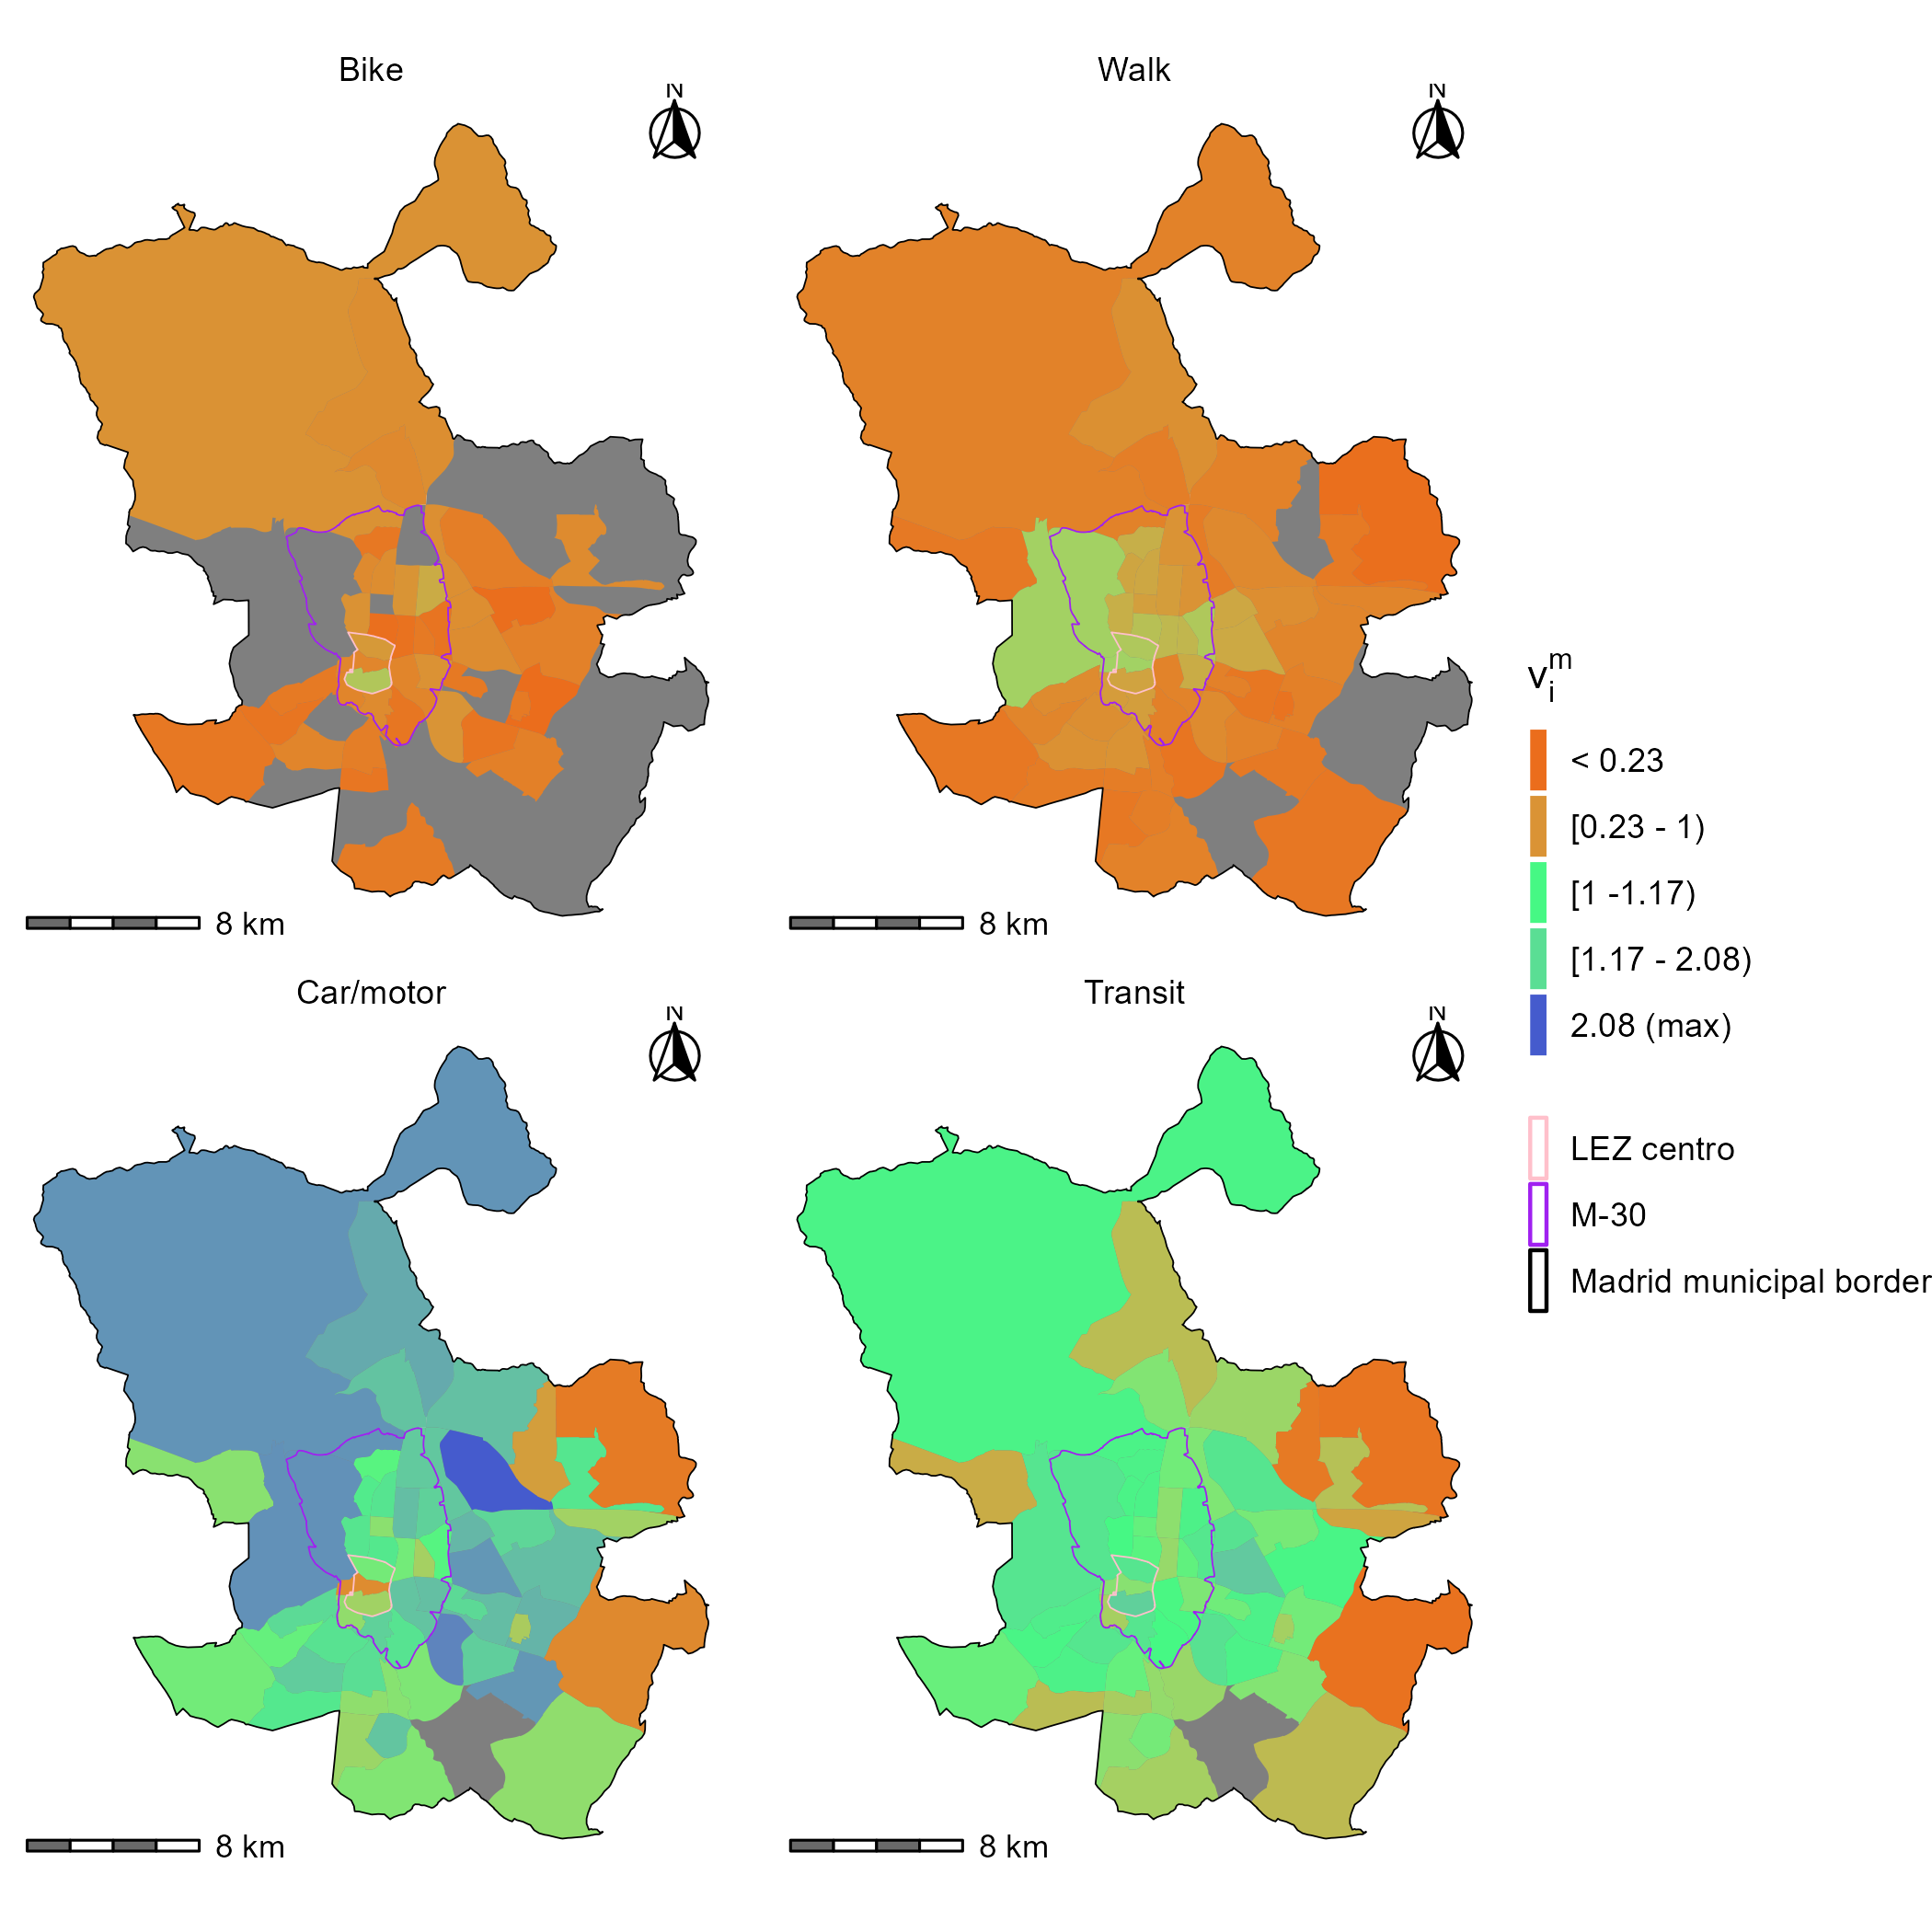
\includegraphics[width=0.85\linewidth]{images/Fig7} 

}

\caption{\label{fig:Fig7} Distribution of spatially available jobs per capita by mode of transportatin ($v_i^m$) represented at the level of TAZ. Grey TAZ have no population that use the mode. Ranges of values in the legend are quintiles. The TAZ shapefile is available from the Community of Madrid open data portal.}\label{fig:SA-per-capita-m-plot}
\end{figure}

Incidentally, \(v_i^m\) values for car within and near LEZ Centro is
close to or below one in Figure \ref{fig:Fig7}, while all non-car modes
have relatively higher \(v_i^m\) values. Since these values are
comparable across regions and over time, Figure \ref{fig:Fig7}
potentially provides a benchmark for quantifying changes in LEZ policies
in the future. As Figure \ref{fig:Fig7} also shows, many areas within
the M-30 have high (white/green) \(v_i^m\) values for car, but the
results for LEZ Centro give reasonable grounds to speculate that a
spatial expansion of the LEZ to include all areas within the M-30 would
likely increase the spatial availability of jobs for transit users,
cyclists and pedestrians.

\hypertarget{discussion-and-conclusions}{%
\section{Discussion and conclusions}\label{discussion-and-conclusions}}

Accessibility measures are an important tool in transportation research
{[}9{]} and are increasingly seen as valuable for planning purposes
{[}4--8{]}. They boast a long history of development, beginning with
Hansen-type \(S_i^m\) measures, with other developments like Shen's
\(a_i^m\), to account for competition/congestion. The more recent
spatial availability measure \(V_i^m\) has in common with these
accessibility indicators that it is a weighted sum of the opportunities
in a region from the perspective of a determined origin \(i\).
Aggregations of opportunities embody principles of gravitational/spatial
interaction modelling that date back to at least H.C. Carey {[}61{]},
and are part of a line of research that includes the work of Ravenstein
{[}62{]}, Reilly {[}63{]}, Stewart {[}64--66{]}, Zipf {[}67,68{]},
Wilson {[}48{]}, and many others. In this way, \(S_i^m\), \(a_i^m\), and
yes, \(V_i^m\), can be interpreted as scores of the potential for
interaction with opportunities in space.

Different accessibility indicators are characterized by how they weight
and aggregate opportunities. Spatial availability's contribution to the
literature is to incorporate a proportional allocation mechanism that
essentially constrains the sums to match the number of opportunities in
the region; in this way it is a singly-constrained accessibility measure
that natively accommodates congestion and competition. The effort with
spatial availability is in line with previous research on proportional
allocation by Paez et al. {[}12{]}. As initially introduced by Soukhov
et al. {[}15{]}, spatial availability was designed for a homogeneous
population traveling by a single mode of transportation. In this paper,
we extended spatial availability for the case of heterogeneous
populations. We discussed this in terms of multiple modes of
transportation, but the framework can accommodate equally well
variations in travel behavior by population segments.

An empirical example using data from Madrid helps to illustrate the
potential of multimodal spatial availability analysis, including its
ability to account for competition for opportunities within and between
modes. Particularly relevant is the fact that spatial availability
scores relate directly to the total number of opportunities in the
region. This makes it possible to compare the results to intuitive
benchmarks, such as opportunities per population, in ways that other
accessibility measures cannot or tend to obfuscate. This comparability
is preserved between regions and over time. The example suggests that
once that opportunities are treated as being finite, restrictions to
travel by car (due to the LEZ) leave more spatially available
opportunities for non-car users. This difference for car travel in
locations within and immediately around the LEZ Centro seems to increase
the number of opportunities spatially available to transit users
(transit being the second most competitive mode), as well as the spatial
availability from the perspective of non-motorised modes. In effect, a
policy such as LEZ seems to help improve the spatial availability
situation of active travel and transit in the parts of the city where it
is implemented.

The purpose of the empirical example is to illustrate the kind of
insights that can be derived from the application of multimodal spatial
availability. But there are some intriguing opportunities for future
research. Accessibility indicators are not designed to work as modal
split models, and yet, in the case of policies that alter the relative
cost of various forms of transportation, one can reasonably expect to
see some shifts between modes. In our empirical example we used data
collected after the introduction of LEZ Centro. However, given a modal
split model to predict model shares, accessibility indicators, including
spatial availability, can be used to investigate changes to the
accessibility landscape. A similar logic can be applied for destination
choice. Our empirical example presented a snapshot of this, and in
future research it may be interesting to investigate changes in spatial
availability \emph{between} policy interventions. The expansion of
Madrid's LEZ to the ring contained by the M-30 presents an excellent
opportunity to do so. Given the intuitive interpretation of spatial
availability scores as fractions of opportunities from the total,
relative and absolute changes in the spatial availability landscape can
be assessed, thus helping to evaluate the implications of policy
interventions.

Our empirical example dealt with differences in travel by mode only, but
it is possible to think of the intersection between mode of travel and
different types of travelers. This would expand the number of
sub-populations in the analysis from, say, \(m=M\) (modes) to
\(m = M\cdot Q\) (modes times population segments), each with their own
characteristic impedance function. Evaluations of this kind will be
especially relevant as LEZ are implemented in cities globally, and the
question of their impact on disadvantaged populations who have become
mobility-restricted increasingly come to the fore {[}51,69,70{]}.

It is worth reiterating that while the focus of this work was on a
multimodal extension of spatial availability, the consideration of
multiple modes is just one case of heterogeneous populations (i.e.,
travel by different modes). The method itself can easily accommodate
other forms of population or opportunity heterogeneity, for example:
variations in rich and poor, young and old, types of opportunities. Like
accessibility measures before it, the potential application of spatial
availability measure are as numerous as potential study contexts.

To close, spatial availability is a singly-constrained accessibility
measure that considers competition, a way of accounting for opportunity
congestion. Spatial availability considers competition by allocating
opportunities (the subject of the single-constraint) to zones based on
zonal proportions. If the demand, supply and travel to opportunities is
spatially uniform, then competition is uniform and spatial availability
will reflect this. It has been suggested that opportunity congestion can
be seen on a continuum, but how it is to be considered within
accessibility research is an ongoing subject of exploration
{[}14,17,18{]}. This is the context in which we present spatial
availability and the multimodal extension.

\hypertarget{author-contributions}{%
\section{Author contributions}\label{author-contributions}}

The authors confirm contribution to the paper as follows: study
conception and design: AS, JTO, JSL, AP.; data collection: AS, JTO,
JSL.; analysis and interpretation of results: AS, JTO, JSL, AP.; draft
manuscript preparation: AS, JSL, AP. All authors reviewed the results
and approved the final version of the manuscript.

\hypertarget{references}{%
\section*{References}\label{references}}
\addcontentsline{toc}{section}{References}

\hypertarget{refs}{}
\begin{CSLReferences}{0}{0}
\leavevmode\vadjust pre{\hypertarget{ref-hansenHowAccessibilityShapes1959}{}}%
\CSLLeftMargin{1. }%
\CSLRightInline{Hansen WG. How accessibility shapes land use. Journal of
the American Institute of Planners. 1959;25: 73--76.
doi:\href{https://doi.org/10.1080/01944365908978307}{10.1080/01944365908978307}}

\leavevmode\vadjust pre{\hypertarget{ref-geursAccessibility2004}{}}%
\CSLLeftMargin{2. }%
\CSLRightInline{Geurs KT, Wee B van. Accessibility evaluation of
land-use and transport strategies: Review and research directions.
Journal of Transport Geography. 2004;12: 127--140. Available:
\href{http://www.sciencedirect.com/science/article/B6VG8-4B28VY7-1/2/61478339c14cab4fa58438ad7b1f4610\%0AC:/Papers/Journal\%20of\%20Transport\%20Geography/Journal\%20of\%20Transport\%20Geography\%20(2004)\%2012\%20(2)\%20127-140.pdf}{http://www.sciencedirect.com/science/article/B6VG8-4B28VY7-1/2/61478339c14cab4fa58438ad7b1f4610
C:/Papers/Journal of Transport Geography/Journal of Transport Geography
(2004) 12 (2) 127-140.pdf}}

\leavevmode\vadjust pre{\hypertarget{ref-paezPositive2012}{}}%
\CSLLeftMargin{3. }%
\CSLRightInline{Paez A, Scott DM, Morency C. Measuring accessibility:
Positive and normative implementations of various accessibility
indicators. Journal of Transport Geography. 2012;25: 141--153.
doi:\href{https://doi.org/10.1016/j.jtrangeo.2012.03.016}{10.1016/j.jtrangeo.2012.03.016}}

\leavevmode\vadjust pre{\hypertarget{ref-handyAccessibility2020}{}}%
\CSLLeftMargin{4. }%
\CSLRightInline{Handy S. Is accessibility an idea whose time has finally
come? Transportation Research Part D: Transport and Environment.
2020;83: 102319. doi:\url{https://doi.org/10.1016/j.trd.2020.102319}}

\leavevmode\vadjust pre{\hypertarget{ref-levinsonTransportAccessManual2020}{}}%
\CSLLeftMargin{5. }%
\CSLRightInline{Levinson D, King D. Transport access manual: {A} guide
for measuring connection between people and places. {University of
Sydney}; 2020. Available:
\url{https://ses.library.usyd.edu.au/handle/2123/23733}}

\leavevmode\vadjust pre{\hypertarget{ref-siddiqToolsTradeAssessing2021}{}}%
\CSLLeftMargin{6. }%
\CSLRightInline{Siddiq F, D. Taylor B. Tools of the trade?: Assessing
the progress of accessibility measures for planning practice. Journal of
the American Planning Association. 2021;87: 497--511.
doi:\href{https://doi.org/10.1080/01944363.2021.1899036}{10.1080/01944363.2021.1899036}}

\leavevmode\vadjust pre{\hypertarget{ref-yanAccessibilityBasedPlanningAddressing2021}{}}%
\CSLLeftMargin{7. }%
\CSLRightInline{Yan X. Toward accessibility-based planning addressing
the myth of travel cost savings. {JOURNAL} {OF} {THE} {AMERICAN}
{PLANNING} {ASSOCIATION}. 2021;87: 409--423.
doi:\href{https://doi.org/10.1080/01944363.2020.1850321}{10.1080/01944363.2020.1850321}}

\leavevmode\vadjust pre{\hypertarget{ref-elGeneidyMaking2022}{}}%
\CSLLeftMargin{8. }%
\CSLRightInline{El-Geneidy A, Levinson D. Making accessibility work in
practice. Transport Reviews. 2022;42: 129--133.
doi:\href{https://doi.org/10.1080/01441647.2021.1975954}{10.1080/01441647.2021.1975954}}

\leavevmode\vadjust pre{\hypertarget{ref-shiLiterature2020}{}}%
\CSLLeftMargin{9. }%
\CSLRightInline{Shi Y, Blainey S, Sun C, Jing P. A literature review on
accessibility using bibliometric analysis techniques. Journal of
Transport Geography. 2020;87: 102810.
doi:\href{https://doi.org/10.1016/j.jtrangeo.2020.102810}{10.1016/j.jtrangeo.2020.102810}}

\leavevmode\vadjust pre{\hypertarget{ref-handyMeasuring1997}{}}%
\CSLLeftMargin{10. }%
\CSLRightInline{Handy S, Niemeier D. Measuring accessibility: An
exploration of issues and alternatives. Environment and Planning A.
1997;29: 1175--1194. }

\leavevmode\vadjust pre{\hypertarget{ref-kwanSpace1998}{}}%
\CSLLeftMargin{11. }%
\CSLRightInline{Kwan MP. Space-time and integral measures of individual
accessibility: A comparative analysis using a point-based framework.
Geographical Analysis. 1998;30: 191--216. Available:
\href{https://ISI:000074579200001\%0AC:/Papers/Geographical\%20Analysis/Geographical\%20Analysis\%20(1998)\%2030\%20(3)\%20191-216.pdf}{ISI:000074579200001
C:/Papers/Geographical Analysis/Geographical Analysis (1998) 30 (3)
191-216.pdf}}

\leavevmode\vadjust pre{\hypertarget{ref-paezDemand2019}{}}%
\CSLLeftMargin{12. }%
\CSLRightInline{Paez A, Higgins CD, Vivona SF. Demand and level of
service inflation in floating catchment area (FCA) methods. PloS one.
2019;14: e0218773.
doi:\href{https://doi.org/10.1371/journal.pone.0218773}{10.1371/journal.pone.0218773}}

\leavevmode\vadjust pre{\hypertarget{ref-wang2SFCAI2SFCAIntegration2021}{}}%
\CSLLeftMargin{13. }%
\CSLRightInline{Wang F. From 2SFCA to i2SFCA: Integration, derivation
and validation. International Journal of Geographical Information
Science. 2021;35: 628--638.
doi:\href{https://doi.org/10.1080/13658816.2020.1811868}{10.1080/13658816.2020.1811868}}

\leavevmode\vadjust pre{\hypertarget{ref-merlinDoesCompetitionMatter2017}{}}%
\CSLLeftMargin{14. }%
\CSLRightInline{Merlin LA, Hu L. Does competition matter in measures of
job accessibility? Explaining employment in los angeles. Journal of
Transport Geography. 2017;64: 77--88.
doi:\href{https://doi.org/10.1016/j.jtrangeo.2017.08.009}{10.1016/j.jtrangeo.2017.08.009}}

\leavevmode\vadjust pre{\hypertarget{ref-soukhovIntroducingSpatialAvailability2023}{}}%
\CSLLeftMargin{15. }%
\CSLRightInline{Soukhov A, Paez A, Higgins CD, Mohamed M. Introducing
spatial availability, a singly-constrained measure of competitive
accessibility \textbar{} {PLOS ONE}. PLOS ONE. 2023; 1--30.
doi:\href{https://\%20doi.org/10.1371/journal.pone.0278468}{https://
doi.org/10.1371/journal.pone.0278468}}

\leavevmode\vadjust pre{\hypertarget{ref-linUsingTransportationProblem2023}{}}%
\CSLLeftMargin{16. }%
\CSLRightInline{Lin J, Cromley G. Using the transportation problem to
build a congestion/threshold constrained spatial accessibility model.
Journal of Transport Geography. 2023;112: 103691.
doi:\href{https://doi.org/10.1016/j.jtrangeo.2023.103691}{10.1016/j.jtrangeo.2023.103691}}

\leavevmode\vadjust pre{\hypertarget{ref-vanweeAccessibilityMeasuresCompetition2001}{}}%
\CSLLeftMargin{17. }%
\CSLRightInline{Van Wee B, Hagoort M, Annema JA. Accessibility measures
with competition. Journal of Transport Geography. 2001;9: 199--208.
doi:\href{https://doi.org/10.1016/S0966-6923(01)00010-2}{10.1016/S0966-6923(01)00010-2}}

\leavevmode\vadjust pre{\hypertarget{ref-kelobonyeMeasuringAccessibilitySpatial2020a}{}}%
\CSLLeftMargin{18. }%
\CSLRightInline{Kelobonye K, Zhou H, McCarney G, Xia J(Cecilia).
Measuring the accessibility and spatial equity of urban services under
competition using the cumulative opportunities measure. Journal of
Transport Geography. 2020;85: 102706.
doi:\href{https://doi.org/10.1016/j.jtrangeo.2020.102706}{10.1016/j.jtrangeo.2020.102706}}

\leavevmode\vadjust pre{\hypertarget{ref-cuiSpatialAccessPublic2020}{}}%
\CSLLeftMargin{19. }%
\CSLRightInline{Cui B, Boisjoly G, Wasfi R, Orpana H, Manaugh K, Buliung
R, et al. Spatial access by public transport and likelihood of
healthcare consultations at hospitals. {TRANSPORTATION} {RESEARCH}
{RECORD}. 2020;2674: 188--198.
doi:\href{https://doi.org/10.1177/0361198120952793}{10.1177/0361198120952793}}

\leavevmode\vadjust pre{\hypertarget{ref-maoMeasuringSpatialAccessibility2013}{}}%
\CSLLeftMargin{20. }%
\CSLRightInline{Mao L, Nekorchuk D. Measuring spatial accessibility to
healthcare for populations with multiple transportation modes. Health \&
Place. 2013;24: 115--122.
doi:\href{https://doi.org/10.1016/j.healthplace.2013.08.008}{10.1016/j.healthplace.2013.08.008}}

\leavevmode\vadjust pre{\hypertarget{ref-josephMeasuringPotentialPhysical1982}{}}%
\CSLLeftMargin{21. }%
\CSLRightInline{Joseph AE, Bantock PR. Measuring potential physical
accessibility to general practitioners in rural areas: A method and case
study. Social Science \& Medicine. 1982;16: 85--90.
doi:\href{https://doi.org/10.1016/0277-9536(82)90428-2}{10.1016/0277-9536(82)90428-2}}

\leavevmode\vadjust pre{\hypertarget{ref-higgsModellingSpatialAccess2017}{}}%
\CSLLeftMargin{22. }%
\CSLRightInline{Higgs G, Zahnow R, Corcoran J, Langford M, Fry R.
Modelling spatial access to general practitioner surgeries: Does public
transport availability matter? {JOURNAL} {OF} {TRANSPORT} \& {HEALTH}.
2017;6: 143--154.
doi:\href{https://doi.org/10.1016/j.jth.2017.05.361}{10.1016/j.jth.2017.05.361}}

\leavevmode\vadjust pre{\hypertarget{ref-weibullAxiomaticApproachMeasurement1976}{}}%
\CSLLeftMargin{23. }%
\CSLRightInline{Weibull JW. An axiomatic approach to the measurement of
accessibility. Regional Science and Urban Economics. 1976;6: 357--379.
doi:\href{https://doi.org/10.1016/0166-0462(76)90031-4}{10.1016/0166-0462(76)90031-4}}

\leavevmode\vadjust pre{\hypertarget{ref-shenLocationCharacteristicsInnercity1998}{}}%
\CSLLeftMargin{24. }%
\CSLRightInline{Shen Q. Location characteristics of inner-city
neighborhoods and employment accessibility of low-wage workers. Environ
Plann B. 1998;25: 345--365.
doi:\href{https://doi.org/10.1068/b250345}{10.1068/b250345}}

\leavevmode\vadjust pre{\hypertarget{ref-liMeasuringMultiactivitiesAccessibility2024a}{}}%
\CSLLeftMargin{25. }%
\CSLRightInline{Li C, Wang J. Measuring multi-activities accessibility
and equity with accessibility-oriented development strategies.
Transportation Research Part D: Transport and Environment. 2024;126:
104035.
doi:\href{https://doi.org/10.1016/j.trd.2023.104035}{10.1016/j.trd.2023.104035}}

\leavevmode\vadjust pre{\hypertarget{ref-wuWillOpeningCommunity2020}{}}%
\CSLLeftMargin{26. }%
\CSLRightInline{Wu J, Chen H, Wang H, He Q, Zhou K. Will the opening
community policy improve the equity of green accessibility and in what
ways? --- response based on a 2-step floating catchment area method and
genetic algorithm. Journal of Cleaner Production. 2020;263: 121454.
doi:\href{https://doi.org/10.1016/j.jclepro.2020.121454}{10.1016/j.jclepro.2020.121454}}

\leavevmode\vadjust pre{\hypertarget{ref-chenEnhancingTwoStepFloating2019}{}}%
\CSLLeftMargin{27. }%
\CSLRightInline{Chen X. Enhancing the two-step floating catchment area
model for community food access mapping: Case of the supplemental
nutrition assistance program. The Professional Geographer. 2019;71:
668--680.
doi:\href{https://doi.org/10.1080/00330124.2019.1578978}{10.1080/00330124.2019.1578978}}

\leavevmode\vadjust pre{\hypertarget{ref-luoMeasuresSpatialAccessibility2003}{}}%
\CSLLeftMargin{28. }%
\CSLRightInline{Luo W, Wang F. Measures of spatial accessibility to
health care in a {GIS} environment: Synthesis and a case study in the
chicago region. Environ Plann B Plann Des. 2003;30: 865--884.
doi:\href{https://doi.org/10.1068/b29120}{10.1068/b29120}}

\leavevmode\vadjust pre{\hypertarget{ref-paezHealth2010}{}}%
\CSLLeftMargin{29. }%
\CSLRightInline{Páez A, Mercado R, Farber S, Morency C, Roorda M.
Accessibility to health care facilities in montreal island: An
application of relative accessibility indicators from the perspective of
senior and non-senior residents. International Journal of Health
Geographics. 2010;9: 1--9. }

\leavevmode\vadjust pre{\hypertarget{ref-moniruzzamanMode2013}{}}%
\CSLLeftMargin{30. }%
\CSLRightInline{Moniruzzaman M, Páez A, Nurul Habib KM, Morency C. Mode
use and trip length of seniors in montreal. Journal of Transport
Geography. 2013;30: 89--99.
doi:\url{http://dx.doi.org/10.1016/j.jtrangeo.2013.03.007}}

\leavevmode\vadjust pre{\hypertarget{ref-reyesWalking2014}{}}%
\CSLLeftMargin{31. }%
\CSLRightInline{Reyes M, Paez A, Morency C. Walking accessibility to
urban parks by children: A case study of montreal. Landscape and Urban
Planning. 2014;125: 38--47.
doi:\href{https://doi.org/10.1016/j.landurbplan.2014.02.002}{10.1016/j.landurbplan.2014.02.002}}

\leavevmode\vadjust pre{\hypertarget{ref-paezJobs2013}{}}%
\CSLLeftMargin{32. }%
\CSLRightInline{Páez A, Farber S, Mercado R, Roorda M, Morency C. Jobs
and the single parent: An analysis of accessibility to employment in
toronto. Urban Geography. 2013;34: 815--842.
doi:\href{https://doi.org/10.1080/02723638.2013.778600}{10.1080/02723638.2013.778600}}

\leavevmode\vadjust pre{\hypertarget{ref-wuUnifyingAccess2020}{}}%
\CSLLeftMargin{33. }%
\CSLRightInline{Wu H, Levinson D. Unifying access. Transportation
Research Part D: Transport and Environment. 2020;83: 102355.
doi:\href{https://doi.org/10.1016/j.trd.2020.102355}{10.1016/j.trd.2020.102355}}

\leavevmode\vadjust pre{\hypertarget{ref-tahmasbiMultimodalAccessibilitybasedEquity2019}{}}%
\CSLLeftMargin{34. }%
\CSLRightInline{Tahmasbi B, Mansourianfar MH, Haghshenas H, Kim I.
Multimodal accessibility-based equity assessment of urban public
facilities distribution. Sustainable Cities and Society. 2019;49:
101633.
doi:\href{https://doi.org/10.1016/j.scs.2019.101633}{10.1016/j.scs.2019.101633}}

\leavevmode\vadjust pre{\hypertarget{ref-lunkeModalAccessibilityDisparities2022}{}}%
\CSLLeftMargin{35. }%
\CSLRightInline{Lunke EB. Modal accessibility disparities and transport
poverty in the oslo region. Transportation Research Part D: Transport
and Environment. 2022;103: 103171.
doi:\href{https://doi.org/10.1016/j.trd.2022.103171}{10.1016/j.trd.2022.103171}}

\leavevmode\vadjust pre{\hypertarget{ref-paezRelative2010}{}}%
\CSLLeftMargin{36. }%
\CSLRightInline{Paez A, Mercado RG, Farber S, Morency C, Roorda M.
Relative accessibility deprivation indicators for urban settings:
Definitions and application to food deserts in montreal. Urban Studies.
2010;47: 1415--1438.
doi:\href{https://doi.org/10.1177/0042098009353626}{10.1177/0042098009353626}}

\leavevmode\vadjust pre{\hypertarget{ref-campbell2019accessibility}{}}%
\CSLLeftMargin{37. }%
\CSLRightInline{Campbell KB, Rising JA, Klopp JM, Mbilo JM.
Accessibility across transport modes and residential developments in
nairobi. Journal of Transport Geography. 2019;74: 77--90. }

\leavevmode\vadjust pre{\hypertarget{ref-maharjanSpatialEquityModal2022}{}}%
\CSLLeftMargin{38. }%
\CSLRightInline{Maharjan S, Tilahun N, Ermagun A. Spatial equity of
modal access gap to multiple destination types across chicago. Journal
of Transport Geography. 2022;104: 103437.
doi:\href{https://doi.org/10.1016/j.jtrangeo.2022.103437}{10.1016/j.jtrangeo.2022.103437}}

\leavevmode\vadjust pre{\hypertarget{ref-grengsJobAccessibilityModal2010}{}}%
\CSLLeftMargin{39. }%
\CSLRightInline{Grengs J. Job accessibility and the modal mismatch in
detroit. Journal of Transport Geography. 2010;18: 42--54.
doi:\href{https://doi.org/10.1016/j.jtrangeo.2009.01.012}{10.1016/j.jtrangeo.2009.01.012}}

\leavevmode\vadjust pre{\hypertarget{ref-kawabataJobAccessibilityIndicator2006}{}}%
\CSLLeftMargin{40. }%
\CSLRightInline{Kawabata M, Shen Q. Job accessibility as an indicator of
auto-oriented urban structure: A comparison of boston and los angeles
with tokyo. Environ Plann B Plann Des. 2006;33: 115--130.
doi:\href{https://doi.org/10.1068/b31144}{10.1068/b31144}}

\leavevmode\vadjust pre{\hypertarget{ref-kwokUseModalAccessibility2004}{}}%
\CSLLeftMargin{41. }%
\CSLRightInline{Kwok RCW, Yeh AGO. The use of modal accessibility gap as
an indicator for sustainable transport development. Environ Plan A.
2004;36: 921--936.
doi:\href{https://doi.org/10.1068/a3673}{10.1068/a3673}}

\leavevmode\vadjust pre{\hypertarget{ref-morrisAccessibilityIndicatorsTransport1979}{}}%
\CSLLeftMargin{42. }%
\CSLRightInline{Morris JM, Dumble PL, Wigan MR. Accessibility indicators
for transport planning. Transportation Research Part A: General.
1979;13: 91--109.
doi:\href{https://doi.org/10.1016/0191-2607(79)90012-8}{10.1016/0191-2607(79)90012-8}}

\leavevmode\vadjust pre{\hypertarget{ref-liottaPlanning2020}{}}%
\CSLLeftMargin{43. }%
\CSLRightInline{Liotta C, Kervinio Y, Levrel H, Tardieu L. Planning for
environmental justice - reducing well-being inequalities through urban
greening. Environmental Science \& Policy. 2020;112: 47--60.
doi:\url{https://doi.org/10.1016/j.envsci.2020.03.017}}

\leavevmode\vadjust pre{\hypertarget{ref-OECDFrameworks2013}{}}%
\CSLLeftMargin{44. }%
\CSLRightInline{OECD. Frameworks and sector policies for urban
development in chile. OECD urban policy reviews, chile 2013. 2013.
doi:\url{http://dx.doi.org/10.1787/9789264191808-en}}

\leavevmode\vadjust pre{\hypertarget{ref-laraSpace2015}{}}%
\CSLLeftMargin{45. }%
\CSLRightInline{Lara-Valencia F, García-Pérez H. Space for equity:
Socioeconomic variations in the provision of public parks in hermosillo,
mexico. Local Environment. 2015;20: 350--368.
doi:\href{https://doi.org/10.1080/13549839.2013.857647}{10.1080/13549839.2013.857647}}

\leavevmode\vadjust pre{\hypertarget{ref-martensFair2021}{}}%
\CSLLeftMargin{46. }%
\CSLRightInline{Martens K, Golub A. A fair distribution of
accessibility: Interpreting civil rights regulations for regional
transportation plans. Journal of Planning Education and Research.
2021;41: 425--444.
doi:\href{https://doi.org/10.1177/0739456x18791014}{10.1177/0739456x18791014}}

\leavevmode\vadjust pre{\hypertarget{ref-taoInvestigatingImpactsPublic2020a}{}}%
\CSLLeftMargin{47. }%
\CSLRightInline{Tao Z, Zhou J, Lin X, Chao H, Li G. Investigating the
impacts of public transport on job accessibility in {Shenzhen}, {China}:
A multi-modal approach. Land Use Policy. 2020;99: 105025.
doi:\href{https://doi.org/10.1016/j.landusepol.2020.105025}{10.1016/j.landusepol.2020.105025}}

\leavevmode\vadjust pre{\hypertarget{ref-wilsonFamilty1971}{}}%
\CSLLeftMargin{48. }%
\CSLRightInline{Wilson AG. A family of spatial interaction models, and
associated developments. Environment and Planning A. 1971;3: 1--32. }

\leavevmode\vadjust pre{\hypertarget{ref-carpentieriMultimodalAccessibilityPrimary2020}{}}%
\CSLLeftMargin{49. }%
\CSLRightInline{Carpentieri G, Guida C, Masoumi HE. Multimodal
{Accessibility} to {Primary Health Services} for the {Elderly}: {A Case
Study} of {Naples}, {Italy}. Sustainability. 2020;12: 781.
doi:\href{https://doi.org/10.3390/su12030781}{10.3390/su12030781}}

\leavevmode\vadjust pre{\hypertarget{ref-margaryanLowEmissionZones2021}{}}%
\CSLLeftMargin{50. }%
\CSLRightInline{Margaryan S. Low emission zones and population health.
Journal of Health Economics. 2021;76: 102402.
doi:\href{https://doi.org/10.1016/j.jhealeco.2020.102402}{10.1016/j.jhealeco.2020.102402}}

\leavevmode\vadjust pre{\hypertarget{ref-verbeekJustManagementUrban2022}{}}%
\CSLLeftMargin{51. }%
\CSLRightInline{Verbeek T, Hincks S. The {``just''} management of urban
air pollution? A geospatial analysis of low emission zones in brussels
and london. Applied Geography. 2022;140: 102642.
doi:\href{https://doi.org/10.1016/j.apgeog.2022.102642}{10.1016/j.apgeog.2022.102642}}

\leavevmode\vadjust pre{\hypertarget{ref-tarrinoortizAnalyzingImpactLow2022}{}}%
\CSLLeftMargin{52. }%
\CSLRightInline{Tarriño-Ortiz J, Gómez J, Soria-Lara JA, Vassallo JM.
Analyzing the impact of low emission zones on modal shift. Sustainable
Cities and Society. 2022;77: 103562.
doi:\href{https://doi.org/10.1016/j.scs.2021.103562}{10.1016/j.scs.2021.103562}}

\leavevmode\vadjust pre{\hypertarget{ref-comunidaddemadridResultadosEDM20182020}{}}%
\CSLLeftMargin{53. }%
\CSLRightInline{Comunidad de Madrid. Resultados de la {EDM} 2018 - Datos
Abiertos. 2020 {[}cited 31 Jul 2023{]}. Available:
\url{https://datos.comunidad.madrid/catalogo/dataset/resultados-edm2018}}

\leavevmode\vadjust pre{\hypertarget{ref-comunidaddemadridzoniEDM20182020}{}}%
\CSLLeftMargin{54. }%
\CSLRightInline{Comunidad de Madrid. Zonificación de transporte ZT208 de
la EDM2018 - Datos Abiertos. 2020 {[}cited 1 Dec 2023{]}. Available:
\url{https://datos.crtm.es/datasets/zonificacionzt208}}

\leavevmode\vadjust pre{\hypertarget{ref-lopez_2017_spatial}{}}%
\CSLLeftMargin{55. }%
\CSLRightInline{Lopez FA, Paez A. Spatial clustering of high-tech
manufacturing and knowledge-intensive service firms in the greater
toronto area. Canadian Geographer-Geographe Canadien. 2017;61: 240--252.
doi:\href{https://doi.org/10.1111/cag.12326}{10.1111/cag.12326}}

\leavevmode\vadjust pre{\hypertarget{ref-horbachov_theoretical_2018}{}}%
\CSLLeftMargin{56. }%
\CSLRightInline{Horbachov P, Svichynskyi S. Theoretical substantiation
of trip length distribution for home-based work trips in urban transit
systems. Journal of Transport and Land Use. 2018;11: 593--632.
Available: \url{https://www.jstor.org/stable/26622420}}

\leavevmode\vadjust pre{\hypertarget{ref-batista_estimation_2019}{}}%
\CSLLeftMargin{57. }%
\CSLRightInline{Batista SFA, Leclercq L, Geroliminis N. Estimation of
regional trip length distributions for the calibration of the aggregated
network traffic models. Transportation Research Part B: Methodological.
2019;122: 192--217.
doi:\href{https://doi.org/10.1016/j.trb.2019.02.009}{10.1016/j.trb.2019.02.009}}

\leavevmode\vadjust pre{\hypertarget{ref-fitdistrplus_2015}{}}%
\CSLLeftMargin{58. }%
\CSLRightInline{Delignette-Muller ML, Dutang C. {fitdistrplus}: An {R}
package for fitting distributions. Journal of Statistical Software.
2015;64: 1--34. Available:
\url{https://www.jstatsoft.org/article/view/v064i04}}

\leavevmode\vadjust pre{\hypertarget{ref-reggianiAccessibilityImpedanceForms2011}{}}%
\CSLLeftMargin{59. }%
\CSLRightInline{Reggiani A, Bucci P, Russo G. Accessibility and
impedance forms: Empirical applications to the german commuting network.
International Regional Science Review. 2011;34: 230--252.
doi:\href{https://doi.org/10.1177/0160017610387296}{10.1177/0160017610387296}}

\leavevmode\vadjust pre{\hypertarget{ref-soukhovTTS2016RDataSet2023}{}}%
\CSLLeftMargin{60. }%
\CSLRightInline{Soukhov A, Páez A. {TTS}2016R: A data set to study
population and employment patterns from the 2016 transportation tomorrow
survey in the greater golden horseshoe area, ontario, canada.
Environment and Planning B: Urban Analytics and City Science. 2023;
23998083221146781.
doi:\href{https://doi.org/10.1177/23998083221146781}{10.1177/23998083221146781}}

\leavevmode\vadjust pre{\hypertarget{ref-careyPriciples1858}{}}%
\CSLLeftMargin{61. }%
\CSLRightInline{Carey HC. Principles of social science. Philadelphia:
J.B. Lippincot; Co.; 1858. }

\leavevmode\vadjust pre{\hypertarget{ref-ravensteinLaws1889}{}}%
\CSLLeftMargin{62. }%
\CSLRightInline{Ravenstein EG. The laws of migration. Journal of the
Royal Statistical Society. 1889;52: 241--305.
doi:\href{https://doi.org/10.2307/2979333}{10.2307/2979333}}

\leavevmode\vadjust pre{\hypertarget{ref-reillyMethods1929}{}}%
\CSLLeftMargin{63. }%
\CSLRightInline{Reilly WJ. Methods for the study of retail
relationships. 1929. }

\leavevmode\vadjust pre{\hypertarget{ref-stewartInverse1941}{}}%
\CSLLeftMargin{64. }%
\CSLRightInline{Stewart JQ. An inverse distance variation for certain
social influences. Science. 1941;93: 89--90. Available:
\url{http://www.jstor.org/stable/1668130}}

\leavevmode\vadjust pre{\hypertarget{ref-stewartSuggested1947}{}}%
\CSLLeftMargin{65. }%
\CSLRightInline{Stewart JQ. Suggested principles of ''social physics''.
Science. 1947;106: 179--180. Available:
\url{http://www.jstor.org/stable/1675368}}

\leavevmode\vadjust pre{\hypertarget{ref-stewartDemographic1948}{}}%
\CSLLeftMargin{66. }%
\CSLRightInline{Stewart JQ. Demographic gravitation: Evidence and
applications. Sociometry. 1948;11: 31--58.
doi:\href{https://doi.org/10.2307/2785468}{10.2307/2785468}}

\leavevmode\vadjust pre{\hypertarget{ref-zipfHypothesis1946}{}}%
\CSLLeftMargin{67. }%
\CSLRightInline{Zipf GK. The p 1 p 2/d hypothesis: The case of railway
express. The Journal of Psychology. 1946;22: 3--8.
doi:\href{https://doi.org/10.1080/00223980.1946.9917292}{10.1080/00223980.1946.9917292}}

\leavevmode\vadjust pre{\hypertarget{ref-zipfIntercity1946}{}}%
\CSLLeftMargin{68. }%
\CSLRightInline{Zipf GK. The P1P2/d hypothesis: On the intercity
movement of persons. American Sociological Review. 1946;11: 677--686.
doi:\href{https://doi.org/10.2307/2087063}{10.2307/2087063}}

\leavevmode\vadjust pre{\hypertarget{ref-devrijNooneVisitsMe2022}{}}%
\CSLLeftMargin{69. }%
\CSLRightInline{De Vrij E, Vanoutrive T. {``No-one visits me anymore''}:
Low emission zones and social exclusion via sustainable transport
policy. 2022 {[}cited 27 Jul 2023{]}. Available:
\url{https://www.tandfonline.com/doi/epdf/10.1080/1523908X.2021.2022465?needAccess=true\&role=button}}

\leavevmode\vadjust pre{\hypertarget{ref-liottaWhatDrivesInequalities2023}{}}%
\CSLLeftMargin{70. }%
\CSLRightInline{Liotta C. What drives inequalities in low emission
zones'impacts on job accessibility? Virtual; 2023.
doi:\href{https://doi.org/10.17605/OSF.IO/9VQU7}{10.17605/OSF.IO/9VQU7}}

\end{CSLReferences}

\nolinenumbers



\end{document}
